La validazione del framework GDM è stata organizzata secondo una sequenza progressiva di esperimenti finalizzata a separare le differenti fonti di errore introdotte dalla pipeline. In particolare, non viene valutata direttamente soltanto la prestazione end-to-end del metodo, poiché un eventuale scostamento rispetto a una discretizzazione di riferimento potrebbe essere attribuito indistintamente alla previsione neurale della mesh, al trasferimento dello stato numerico oppure alla formulazione su mesh mobile.

Per questo motivo il protocollo sperimentale è suddiviso in tre stadi successivi:

\begin{enumerate}
    \item \textbf{Stage A}: validazione statica del problema geometrico, del mesh mover neurale e del filtro deterministico;

    \item \textbf{Stage B}: introduzione della PDE transiente e isolamento dell'errore associato al trasferimento della soluzione tra configurazioni successive della mesh;

    \item \textbf{Stage C}: sostituzione del remapping esplicito con una formulazione ALE continua e verifica indipendente della consistenza geometrica mediante D-GCL.
\end{enumerate}

Questa decomposizione consente di interpretare i risultati del benchmark finale come la combinazione di componenti precedentemente sottoposte a verifiche mirate, evitando di confondere in un'unica misura gli errori introdotti dai differenti moduli del framework.

\subsection{Validazione geometrica statica: Stage A}

\label{subsec:stage_a_results}

Lo Stage A considera esclusivamente il problema di adattamento geometrico. La soluzione fisica è rappresentata mediante campi scalari analitici statici caratterizzati da strutture localizzate, così da valutare la capacità del modello di apprendere la corrispondenza tra informazione locale sul campo e rilocazione dei nodi senza introdurre ancora l'integrazione temporale della PDE.

L'esperimento principale considera tre configurazioni di riferimento:

\begin{itemize}
    \item \textbf{Mesh fissa}: configurazione senza adattamento geometrico;
    \item \textbf{GNN}: configurazione ottenuta mediante lo spostamento prodotto direttamente dalla MeshMover;
    \item \textbf{Oracle}: configurazione ottenuta dalla soluzione numerica del problema variazionale introdotto nella Sezione~\ref{subsec:oracle_formulation}.
\end{itemize}

Nel benchmark principale l'output della GNN viene inoltre sottoposto al Safety Filter. Quando la configurazione prodotta dalla rete è già ammissibile, il filtro risulta trasparente e quindi la configurazione GNN coincide con quella filtrata.

L'errore di rappresentazione viene misurato mediante la norma relativa dell'interpolazione del campo sulla mesh risultante. Contestualmente vengono monitorati il minimo determinante Jacobiano orientato e una misura della qualità geometrica della discretizzazione.

\paragraph{Prestazioni sul test interpolativo.}

Sul test set contenente configurazioni appartenenti alla regione parametrica osservata durante l'addestramento, la mesh fissa presenta un errore medio di interpolazione pari a

\[
(0.19\pm0.11)\times10^{-4}.
\]

La configurazione ottenuta dalla GNN raggiunge

\[
(0.15\pm0.08)\times10^{-4},
\]

mentre l'oracolo variazionale raggiunge

\[
(0.08\pm0.04)\times10^{-4}.
\]

Il recupero del divario rispetto all'oracolo associato alla GNN è pari al $32.4\%$. Il valore minimo del determinante Jacobiano della mesh prodotta dalla GNN è

\[
\min_e J_e = 6.38\times10^{-4},
\]

a fronte del valore iniziale

\[
J_0 = 9.77\times10^{-4}.
\]

In queste configurazioni l'output della GNN risulta già ammissibile rispetto alla soglia geometrica prescritta; di conseguenza, il Safety Filter non modifica lo spostamento. Il comportamento è coerente con il ruolo del filtro, che interviene soltanto quando l'output previsto eccede il limite geometrico imposto.

\paragraph{Generalizzazione sul test extrapolativo.}

Un secondo test considera configurazioni esterne alla regione parametrica utilizzata per l'interpolazione. In questo caso l'errore della mesh fissa cresce a

\[
(0.43\pm0.43)\times10^{-4},
\]

mentre la GNN raggiunge

\[
(0.34\pm0.34)\times10^{-4}.
\]

L'oracolo raggiunge invece

\[
(0.11\pm0.09)\times10^{-4}.
\]

Il recupero del divario rispetto all'oracolo aumenta in questo caso al $45.3\%$. Il minimo Jacobiano prodotto dalla GNN rimane positivo,

\[
\min_e J_e = 6.27\times10^{-4},
\]

mostrando che, nel regime extrapolativo considerato, la configurazione prevista rimane geometricamente ammissibile.

Il confronto evidenzia quindi che la GNN non ricostruisce completamente la configurazione ottenuta dall'ottimizzazione variazionale, ma recupera una parte misurabile del beneficio geometrico dell'adattività sia nel regime interpolativo sia in quello extrapolativo.

\begin{table}[htbp]
\centering
\small
\setlength{\tabcolsep}{4.5pt}
\caption{Risultati dello Stage A sui due split di test. L'errore di interpolazione è espresso in unità $10^{-4}$.}
\label{tab:stage_a_benchmark}
\begin{tabular*}{\linewidth}{@{\extracolsep{\fill}}lcc@{}}
\toprule
Configurazione & Test interpolativo & Test extrapolativo \\
\midrule
Mesh fissa              & $0.19 \pm 0.11$ & $0.43 \pm 0.43$ \\
GNN                     & $0.15 \pm 0.08$ & $0.34 \pm 0.34$ \\
Oracle                  & $0.08 \pm 0.04$ & $0.11 \pm 0.09$ \\
\midrule
Recupero Oracle gap GNN & $32.4\%$        & $45.3\%$ \\
\bottomrule
\end{tabular*}
\end{table}

Le corrispondenti distribuzioni dell'errore e del recupero del divario rispetto all'oracolo sono riportate nelle Figure~\ref{fig:stage_a_error} e~\ref{fig:stage_a_oracle_gap}.

\begin{figure}[H]
    \centering
    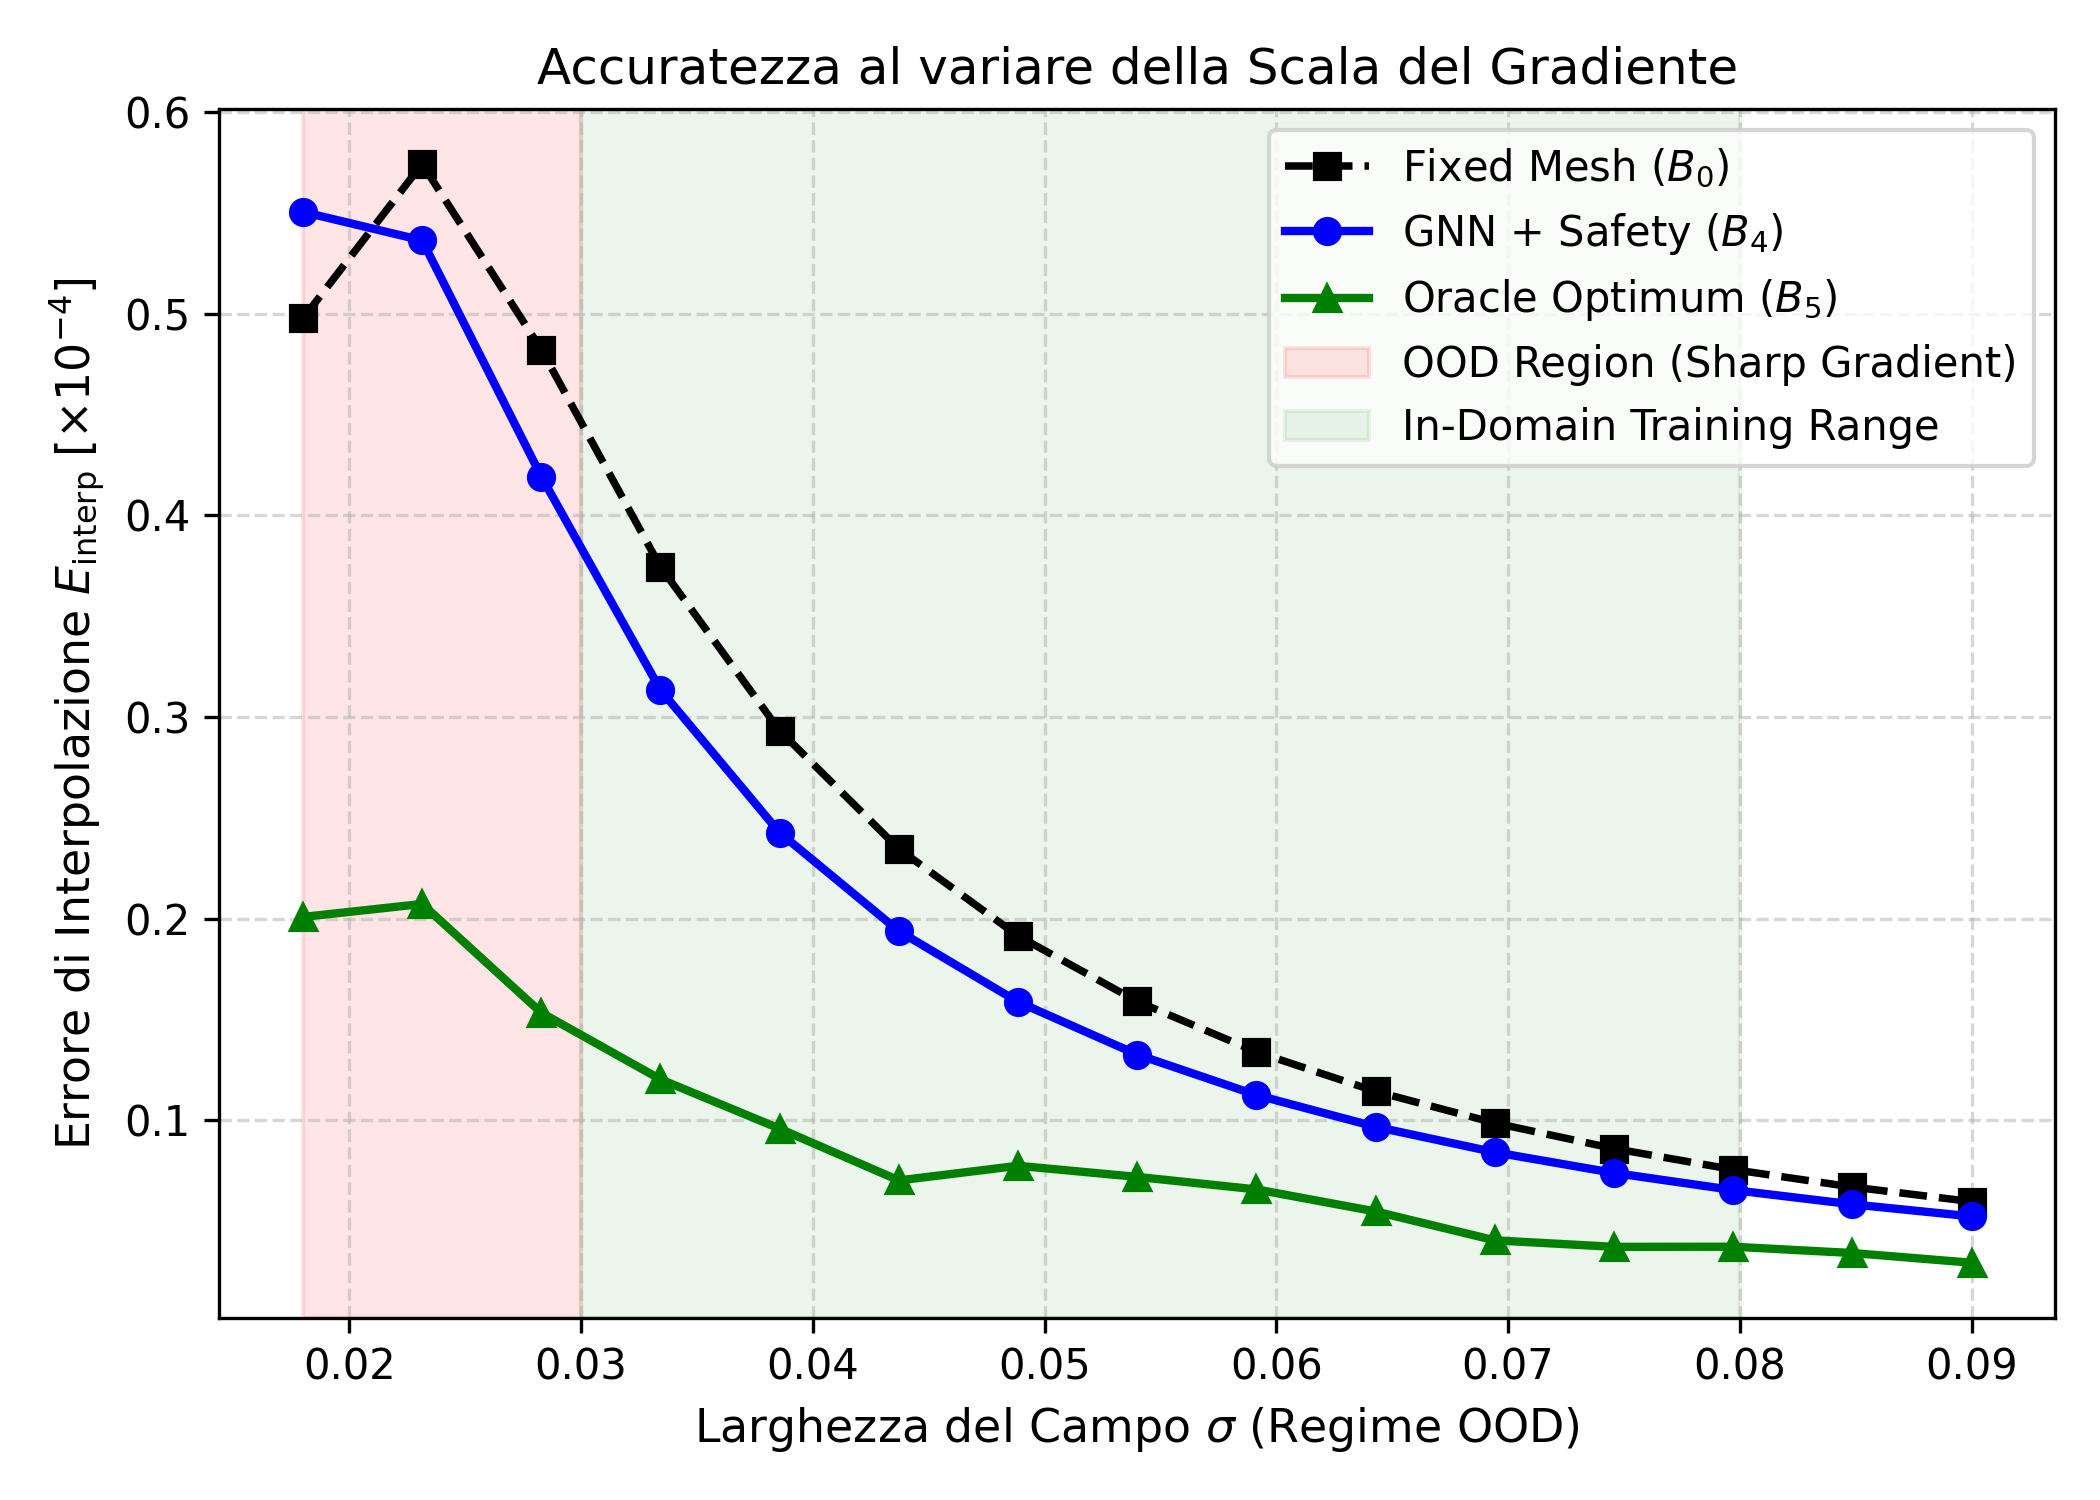
\includegraphics[width=0.95\linewidth]
    {images/stage_a/fig1_error_vs_ood.png}
    \caption{Errore di interpolazione della mesh fissa, della GNN e della configurazione di riferimento sui test interpolativo ed extrapolativo dello Stage A.}
    \label{fig:stage_a_error}
\end{figure}

\begin{figure}[H]
    \centering
    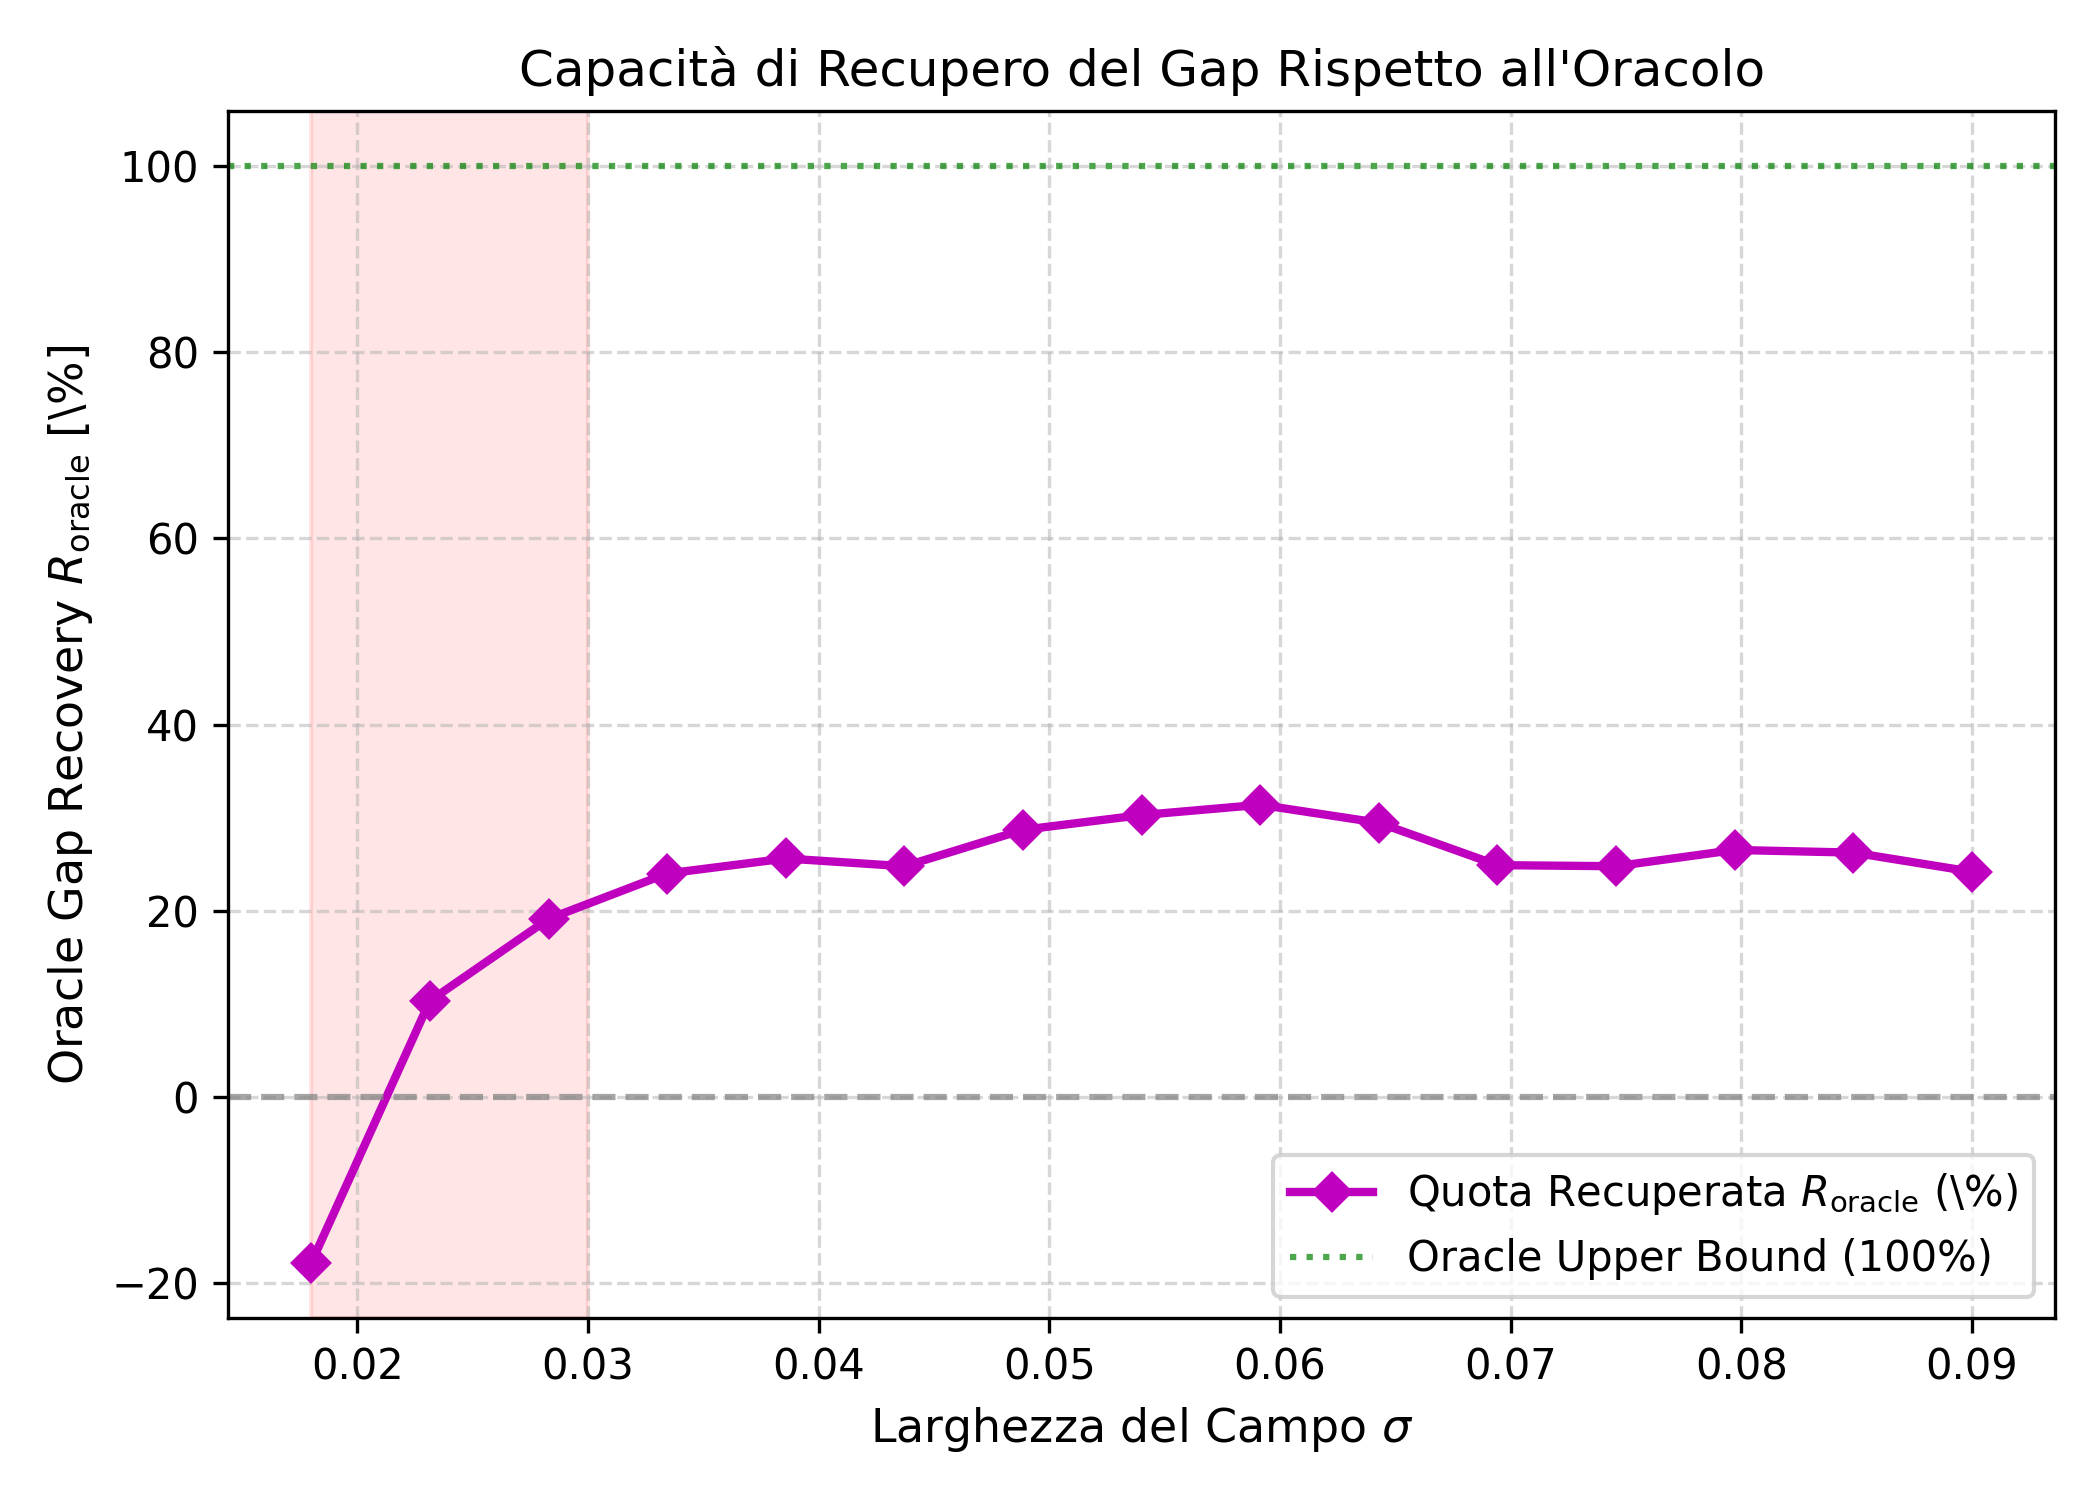
\includegraphics[width=0.85\linewidth]
    {images/stage_a/fig2_oracle_recovery.png}
    \caption{Recupero del divario rispetto all'oracolo ottenuto dalla GNN nei due regimi di test.}
    \label{fig:stage_a_oracle_gap}
\end{figure}

\paragraph{Verifica deterministica del Safety Filter.}

La validazione del filtro viene condotta separatamente dal benchmark principale attraverso uno stress test nel quale lo spostamento prodotto dalla GNN viene moltiplicato per un fattore

\[
k\in\{1,\;1.5,\;2,\;3,\;5,\;10\}.
\]

Per $k\leq3$ la deformazione rimane ammissibile senza alcuna contrazione. Per $k=5$ e $k=10$, invece, la configurazione non filtrata contiene elementi con determinante Jacobiano negativo.

Per $k=5$ il minimo Jacobiano non filtrato scende a

\[
-3.45\times10^{-4},
\]

mentre il Safety Filter determina

\[
\alpha_{\mathrm{global}}\simeq0.678
\]

e porta la configurazione filtrata a una soglia minima pari, entro l'accuratezza numerica del calcolo, a

\[
\min_e J_e \simeq 10^{-4}.
\]

Nel caso più severo, $k=10$, il minimo Jacobiano non filtrato raggiunge

\[
-1.85\times10^{-3},
\]

mentre il fattore ammissibile viene ridotto a

\[
\alpha_{\mathrm{global}}\simeq0.339,
\]

con

\[
\min_e J_e \simeq 10^{-4}.
\]

Il test mostra quindi due comportamenti distinti: per deformazioni già ammissibili il filtro risulta trasparente, mentre per deformazioni che violano il vincolo geometrico riduce automaticamente l'ampiezza dello spostamento fino alla soglia ammissibile. La proprietà è verificata nel modello geometrico considerato, ossia triangoli lineari, traiettoria nodale lineare e soglia prescritta.

\begin{figure}[H]
    \centering
    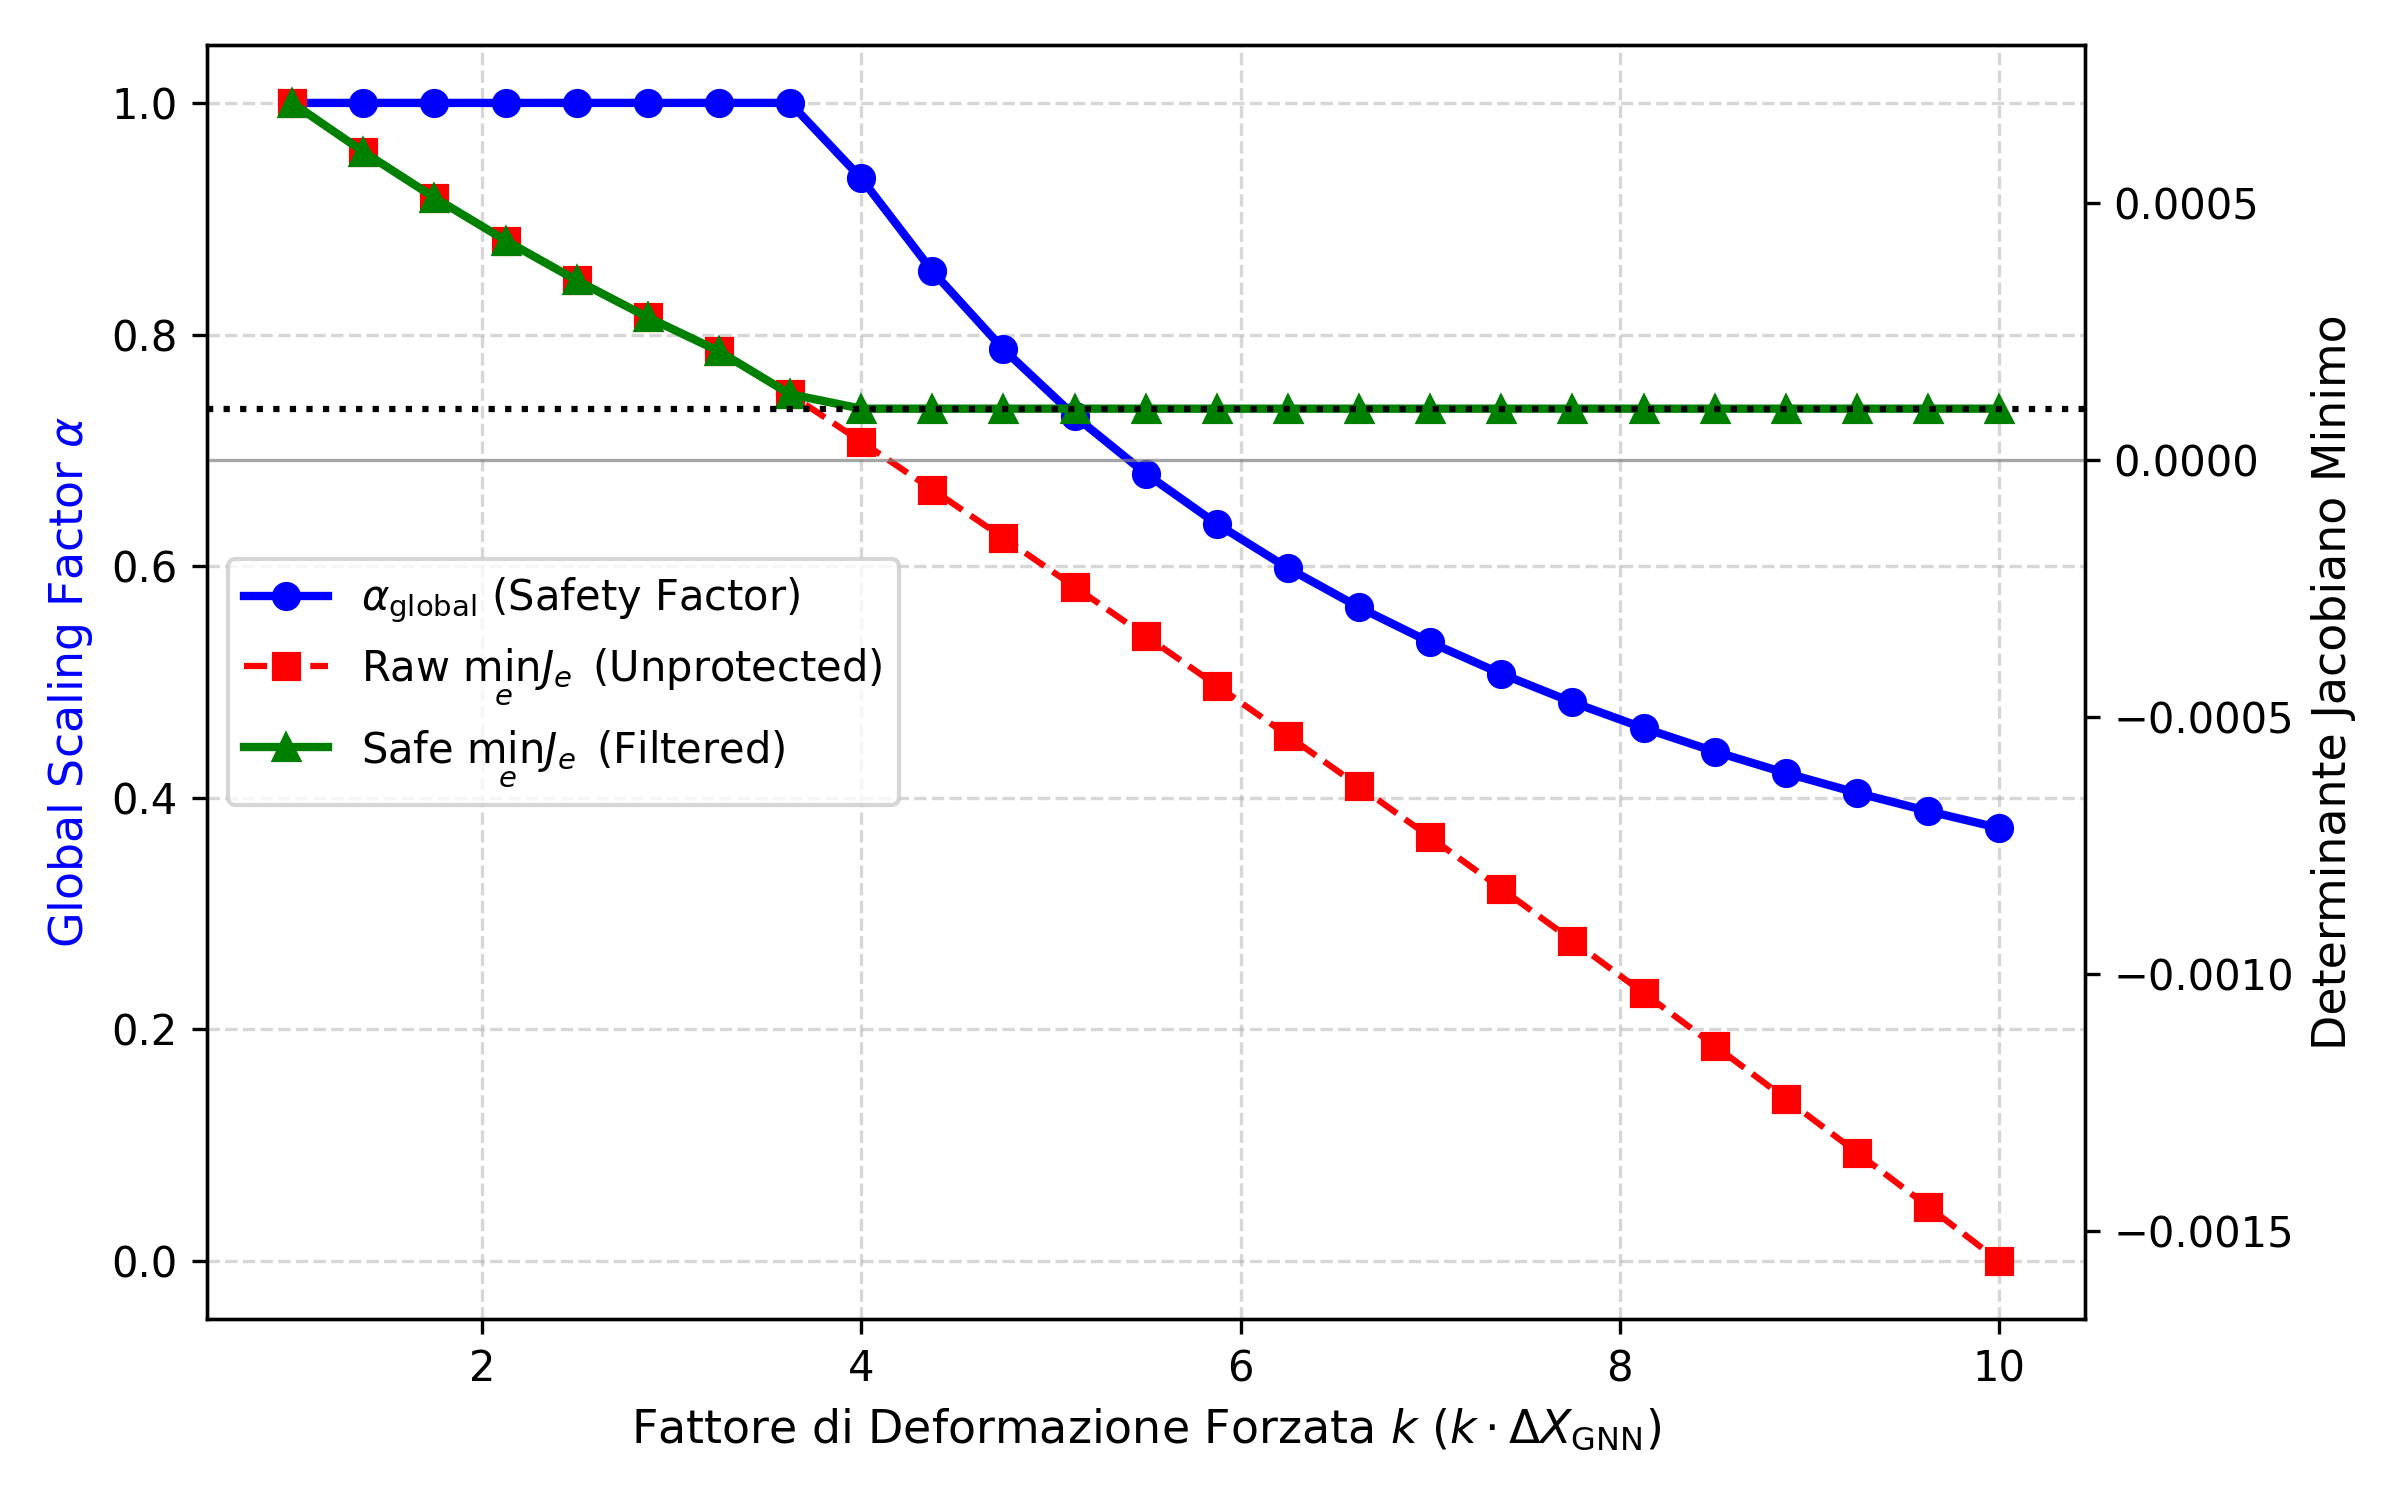
\includegraphics[width=0.85\linewidth]
    {images/stage_a/fig3_safety_curve.png}
    \caption{Attivazione del Safety Filter durante lo stress test geometrico al crescere dell'ampiezza dello spostamento.}
    \label{fig:stage_a_safety}
\end{figure}

La verifica visiva della deformazione prima e dopo il filtraggio è riportata nella Figura~\ref{fig:stage_a_safety_visual}.

\begin{figure}[H]
    \centering
    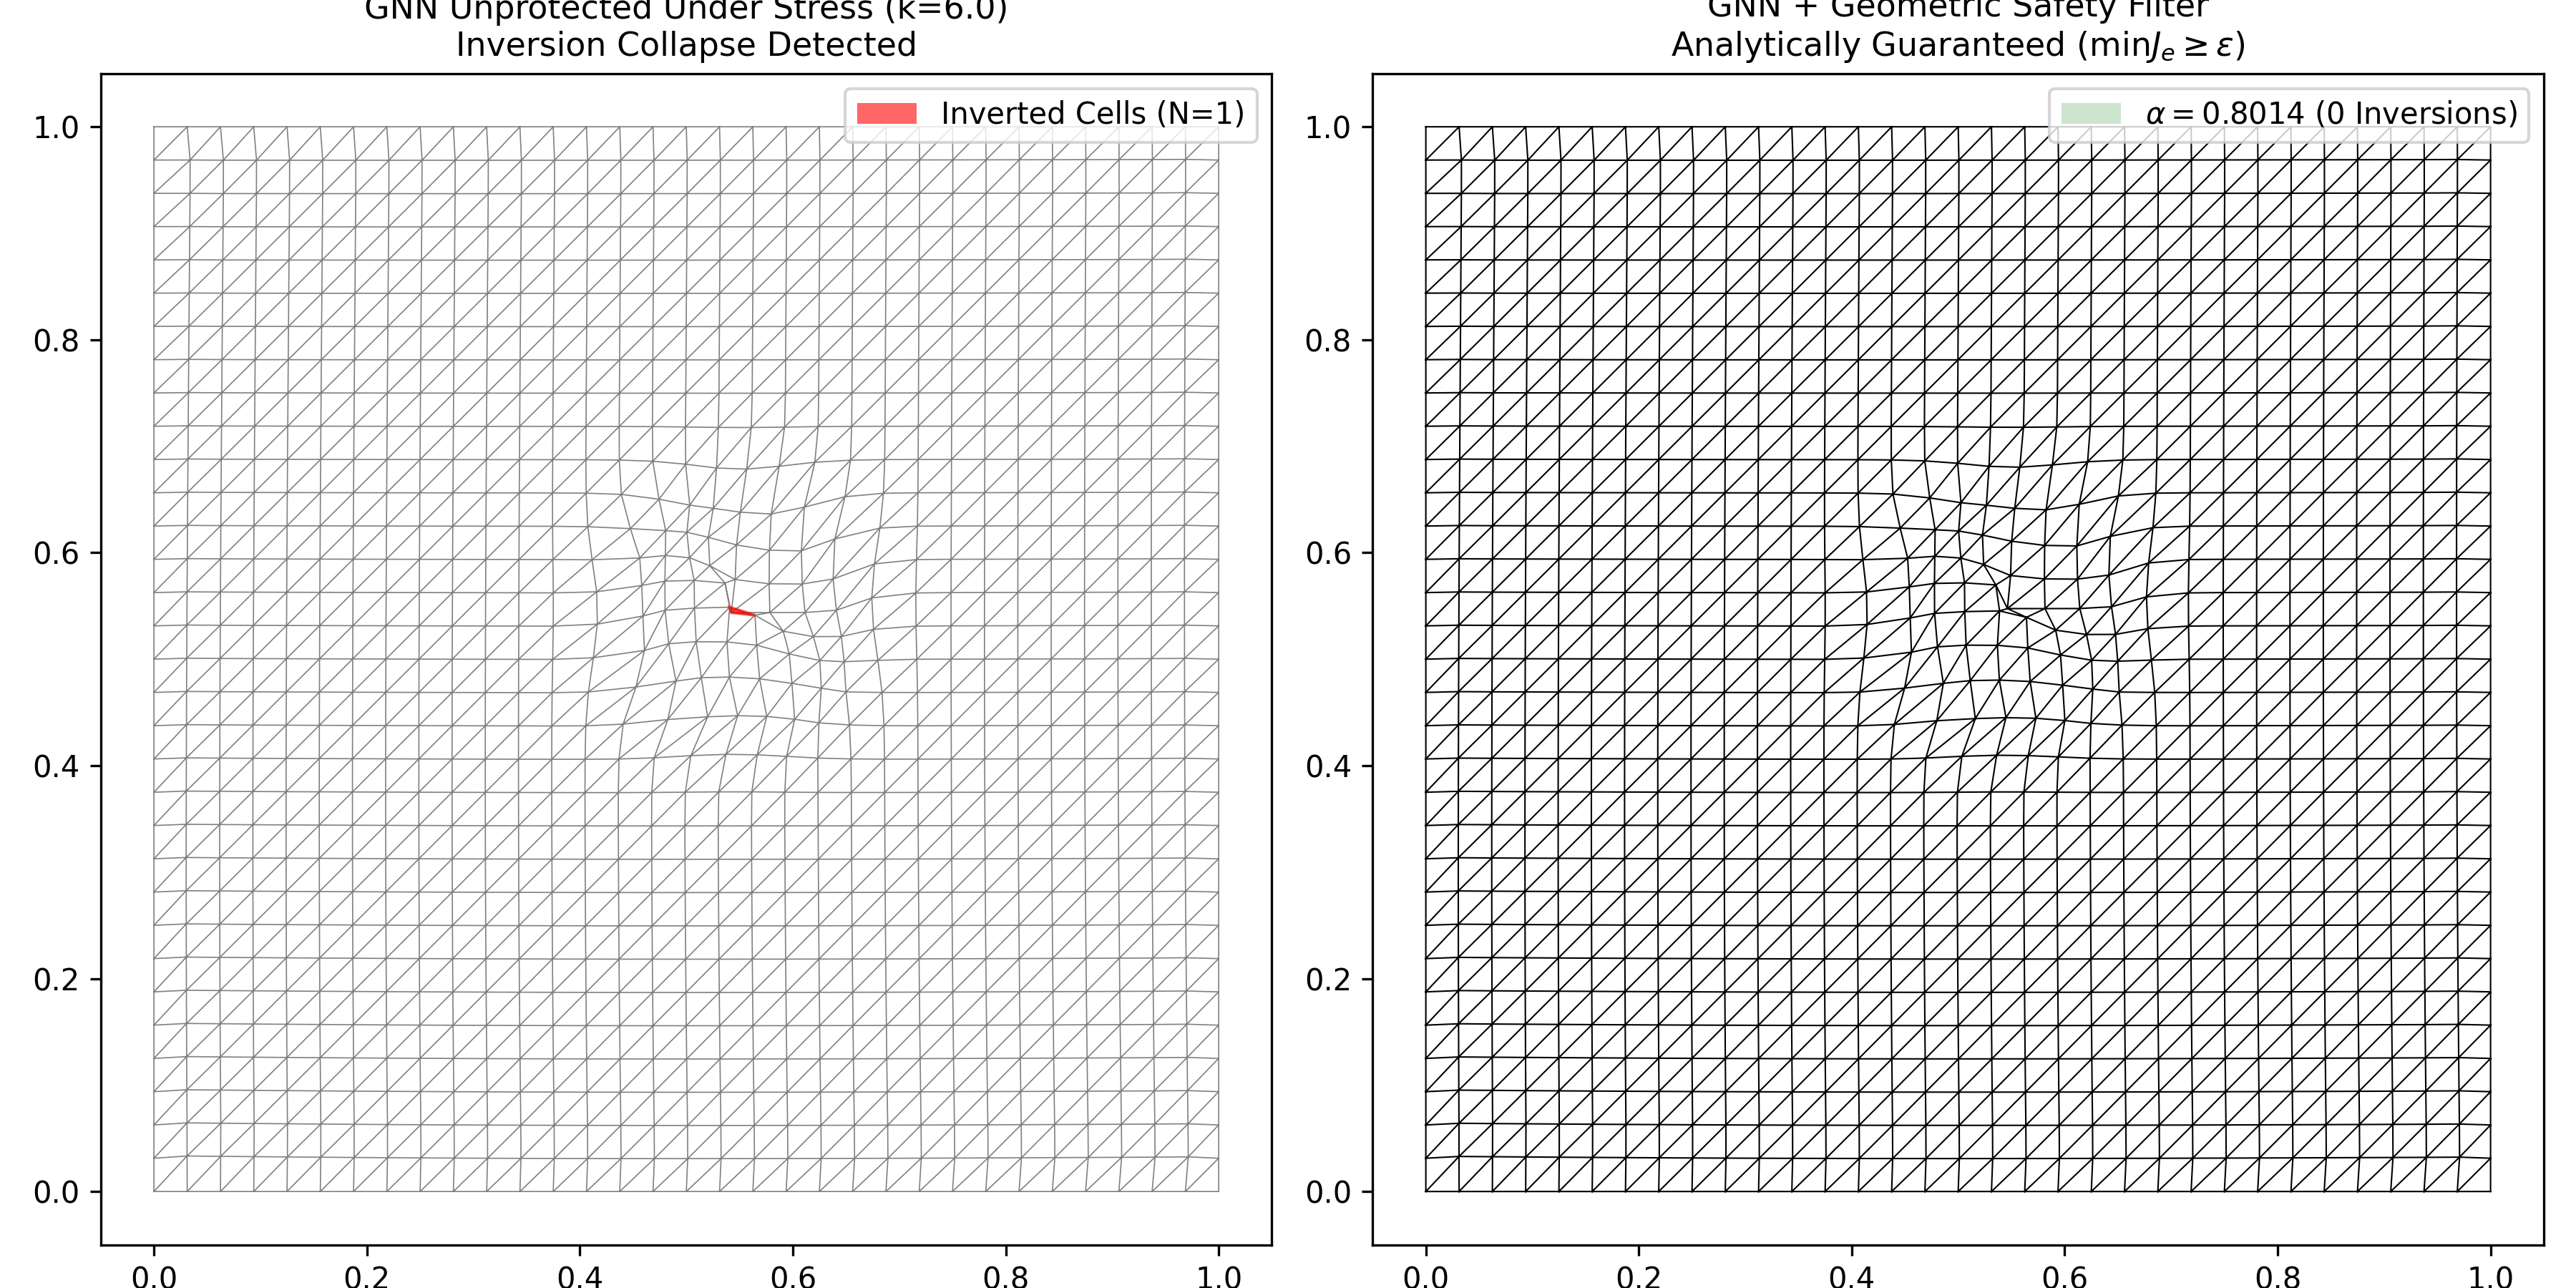
\includegraphics[width=0.95\linewidth]
    {images/stage_a/vis2_safety_stress_visual.png}
    \caption{Esempio di configurazione deformata nello stress test e correzione ottenuta mediante il Safety Filter.}
    \label{fig:stage_a_safety_visual}
\end{figure}

\paragraph{Costo computazionale e scaling.}

Il costo delle tre componenti principali viene misurato utilizzando esclusivamente CPU, così da rendere coerente il confronto tra inferenza GNN, Safety Filter e ottimizzazione variazionale. Il benchmark considera mesh comprese tra $289$ e $4225$ nodi.

Il tempo di inferenza GNN cresce da $15.19$ ms a $184.79$ ms, mentre il costo del Safety Filter passa da $0.23$ ms a $1.39$ ms. L'oracolo variazionale cresce invece da $1.02$ s fino a circa $95.17$ s.

Un fit di potenza sui punti misurati fornisce uno scaling empirico approssimativamente pari a

\[
T_{\mathrm{GNN}}\propto N^{0.93},
\qquad
T_{\mathrm{oracle}}\propto N^{1.69}.
\]

Tali esponenti devono essere interpretati esclusivamente come osservazioni empiriche sul range di dimensioni considerato e non come stime della complessità asintotica generale dei due algoritmi.

\begin{figure}[H]
    \centering
    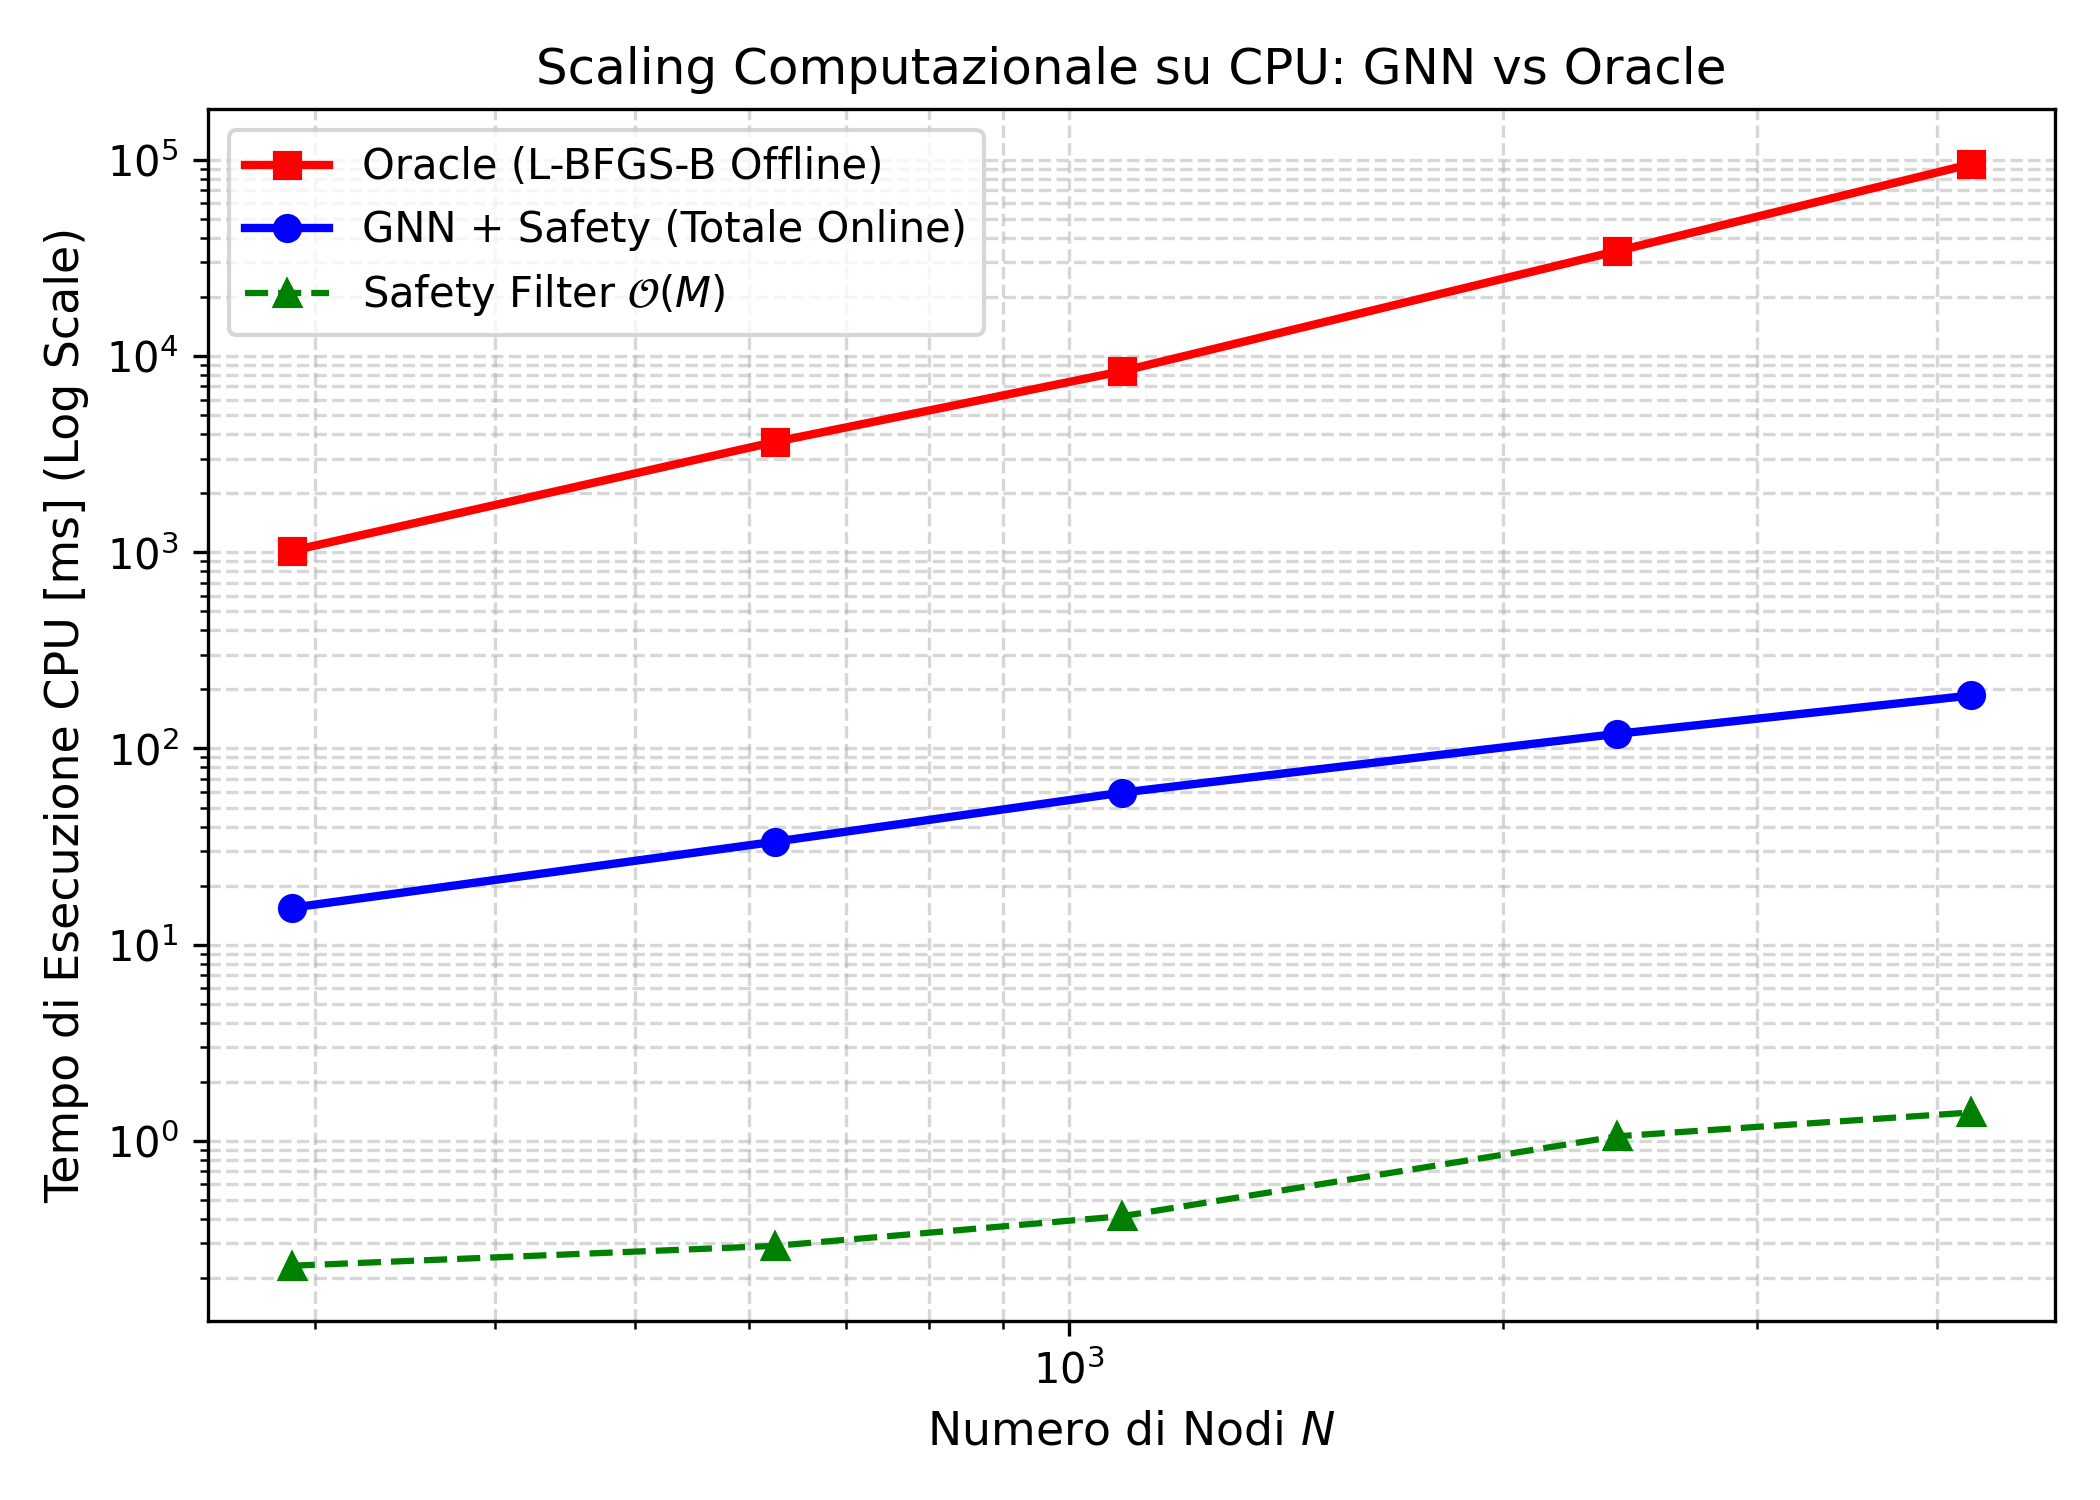
\includegraphics[width=0.90\linewidth]
    {images/stage_a/fig4_runtime_scaling.png}
    \caption{Scaling empirico del costo di inferenza GNN, Safety Filter e ottimizzazione variazionale nello Stage A.}
    \label{fig:stage_a_runtime}
\end{figure}

Nel complesso, lo Stage A mostra che il mesh mover neurale recupera una parte misurabile del beneficio geometrico dell'oracolo e che il controllo geometrico deterministico ha un costo computazionale molto inferiore all'ottimizzazione variazionale nel range di dimensioni testato.

\subsection{Diagnostica dinamica disaccoppiata: Stage B}

\label{subsec:stage_b_diagnostics}

Lo Stage B introduce l'evoluzione temporale della PDE di convezione--diffusione definita nella Sezione~\ref{subsec:pde_governing}. L'obiettivo non è ancora confrontare end-to-end le differenti strategie di mesh motion, ma quantificare separatamente l'impatto del trasferimento dello stato numerico e verificare il comportamento del solutore FEM prima dell'introduzione della formulazione ALE.

La validazione viene pertanto suddivisa in tre gruppi di test:

\begin{enumerate}
    \item verifica indipendente del solutore FEM su mesh fissa;
    \item caratterizzazione del remapping pointwise $P_1$ e della proiezione globale $L^2$;
    \item integrazione della GNN nel problema transiente e studio della frequenza di adattamento.
\end{enumerate}

\subsubsection{Verifica del solutore FEM}

Prima di introdurre il movimento della mesh viene verificata la convergenza del solutore sulla configurazione fissa. Il raffinamento spaziale restituisce ordini di convergenza in norma $L^2$ pari a

\[
1.71,\qquad1.89,\qquad1.97,
\]

mentre per la norma $H^1$ si ottengono

\[
0.80,\qquad0.92,\qquad0.98.
\]

Analogamente, il raffinamento temporale con Backward Euler restituisce ordini

\[
1.04,\qquad1.09,\qquad1.22.
\]

I risultati sono compatibili con gli ordini attesi della discretizzazione $P_1$--Backward Euler discussi nella Sezione~\ref{subsec:fem_discretization}. La verifica stabilisce pertanto che il solutore di riferimento riproduce il comportamento di convergenza previsto prima dell'introduzione del moto della mesh.

\subsubsection{Diagnostica degli operatori di remapping}

La prima verifica riguarda l'esattezza su campi semplici. La proiezione $L^2$ riproduce un campo costante e un campo lineare con errori massimi dell'ordine di

\[
10^{-15},
\]

coerentemente con l'esattezza dello spazio $P_1$ per tali funzioni nel test numerico considerato.

Il successivo studio di convergenza spaziale mostra che entrambi gli operatori convergono al raffinamento della mesh, ma con comportamenti quantitativamente differenti. Per il remapping pointwise $P_1$ vengono osservati ordini sperimentali pari a circa

\[
1.96,\qquad2.00,\qquad2.01,
\]

mentre la proiezione $L^2$ presenta gli ordini

\[
4.12,\qquad2.76,\qquad2.28.
\]

Questi valori sono interpretati esclusivamente come ordini osservati nel benchmark. In particolare, il valore iniziale superiore a $4$ non viene assunto come indicazione di un ordine teorico globale della proiezione $L^2$; l'ultima finestra di raffinamento fornisce un valore pari a $2.28$.

Un secondo test varia l'ampiezza dello spostamento della mesh. Per i fattori di deformazione

\[
\gamma=\{0.1,0.25,0.5,1,2\},
\]

l'errore relativo del remapping pointwise passa da circa $0.20\%$ a $2.96\%$, mentre quello della proiezione $L^2$ rimane compreso tra circa $0.01\%$ e $0.26\%$.

Il test di accumulo a target finale fisso costituisce il confronto più diretto tra i due operatori. Dividendo lo stesso spostamento complessivo in $K=\{1,2,5,10\}$ trasferimenti successivi, il remapping $P_1$ produce errori finali pari a

\[
4.220\%,\quad
5.235\%,\quad
5.779\%,\quad
5.949\%,
\]

con fattori di amplificazione rispettivamente pari a

\[
1.00,\quad1.24,\quad1.37,\quad1.41.
\]

La proiezione $L^2$ produce invece

\[
0.172\%,\quad
0.160\%,\quad
0.364\%,\quad
0.332\%,
\]

con fattori di amplificazione

\[
1.00,\quad0.93,\quad2.12,\quad1.93.
\]

I risultati mostrano che l'applicazione reiterata dell'interpolazione pointwise può produrre un accumulo di errore sensibilmente superiore rispetto alla proiezione globale nel test considerato. La proiezione $L^2$ non elimina tuttavia completamente l'errore introdotto dal trasferimento: i valori misurati rimangono infatti finiti e dipendono dalla configurazione geometrica e dalla frequenza delle proiezioni.

La differenza in accuratezza è accompagnata da un incremento del costo computazionale. Sulla mesh $32\times32$ il tempo medio misurato è circa

\[
27.02\ {\rm ms}
\]

per il remapping $P_1$ e

\[
355.55\ {\rm ms}
\]

per la proiezione $L^2$, corrispondente a un rapporto di costo di circa

\[
13.2\times.
\]

Questa evidenza motiva il passaggio alla formulazione ALE dello Stage C: il problema non consiste soltanto nella scelta del trasferimento più accurato, ma anche nella necessità di eliminare, quando possibile, un'operazione di trasferimento separata che viene ripetuta durante l'evoluzione temporale.

\begin{figure}[H]
    \centering
    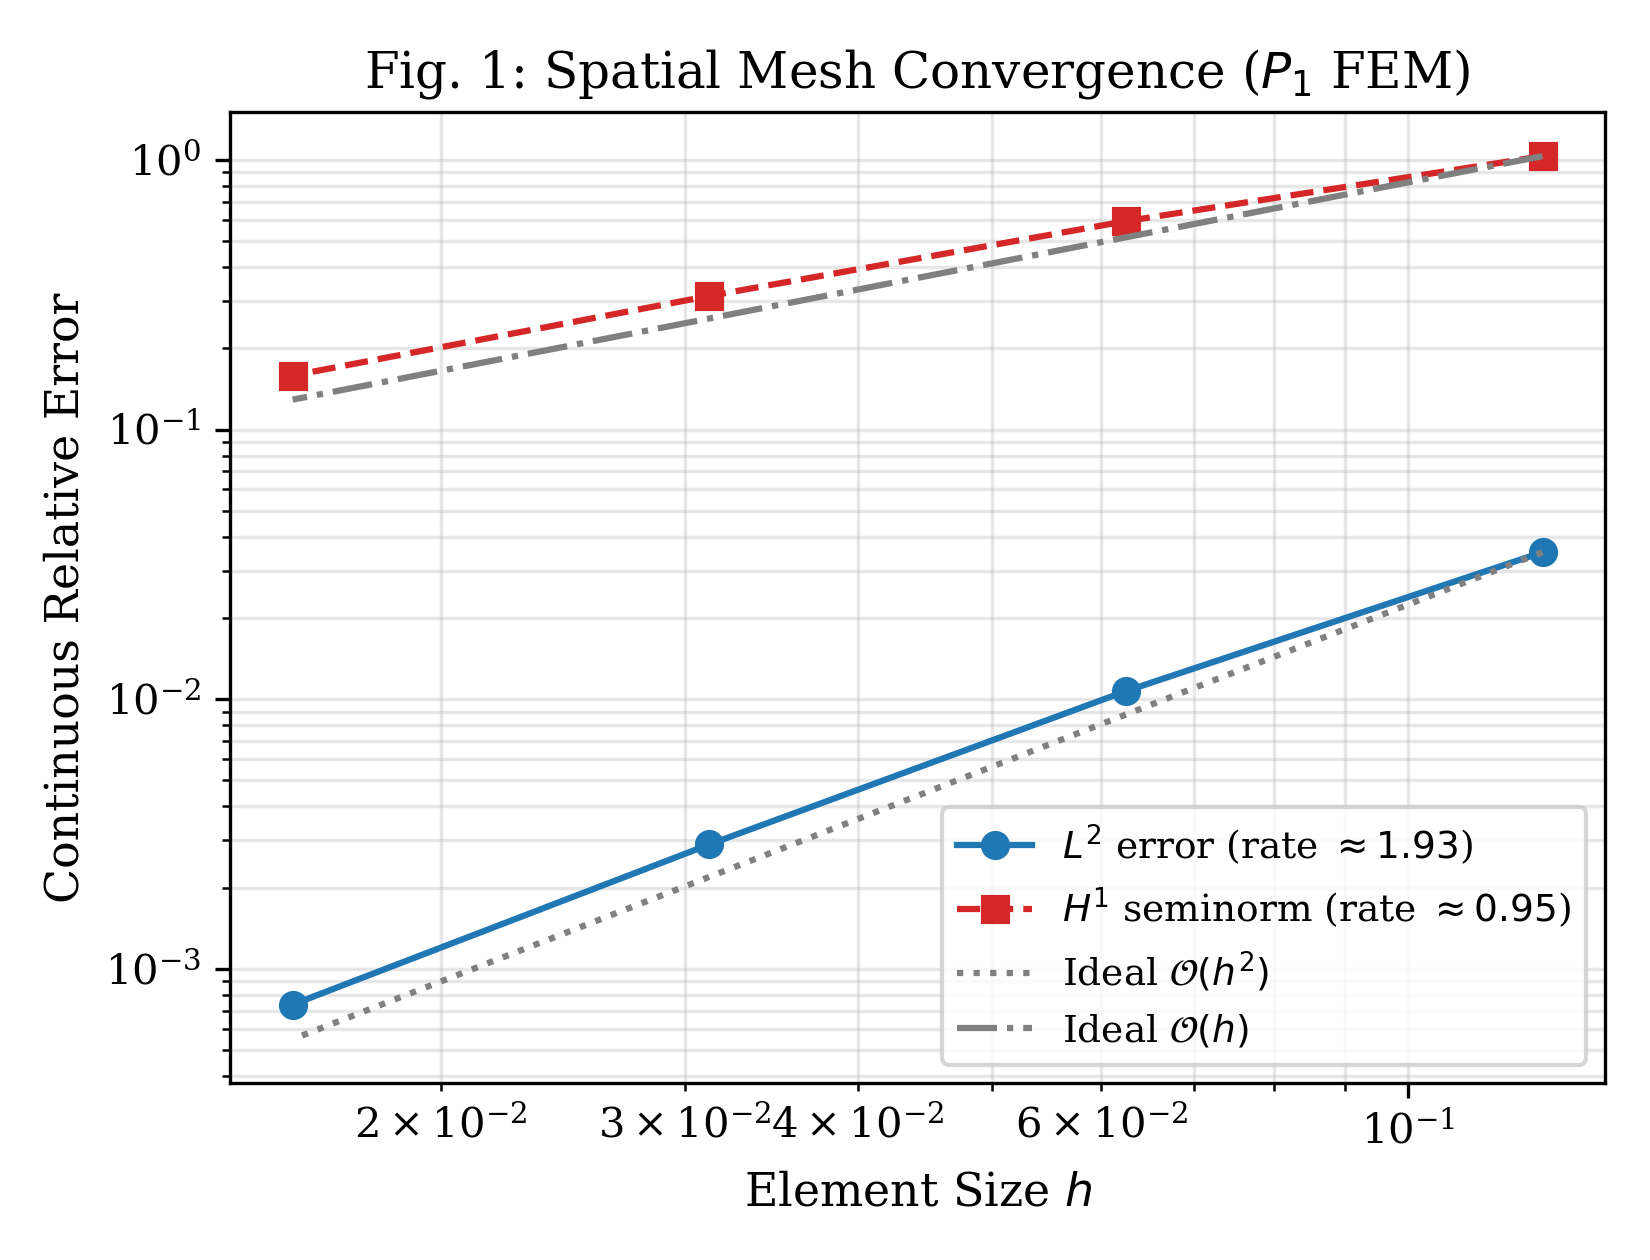
\includegraphics[width=0.90\linewidth]
    {images/stage_b/fig1_spatial_convergence.png}
    \caption{Convergenza spaziale del solutore FEM e confronto tra remapping pointwise $P_1$ e proiezione $L^2$.}
    \label{fig:stage_b_spatial}
\end{figure}

\begin{figure}[H]
    \centering
    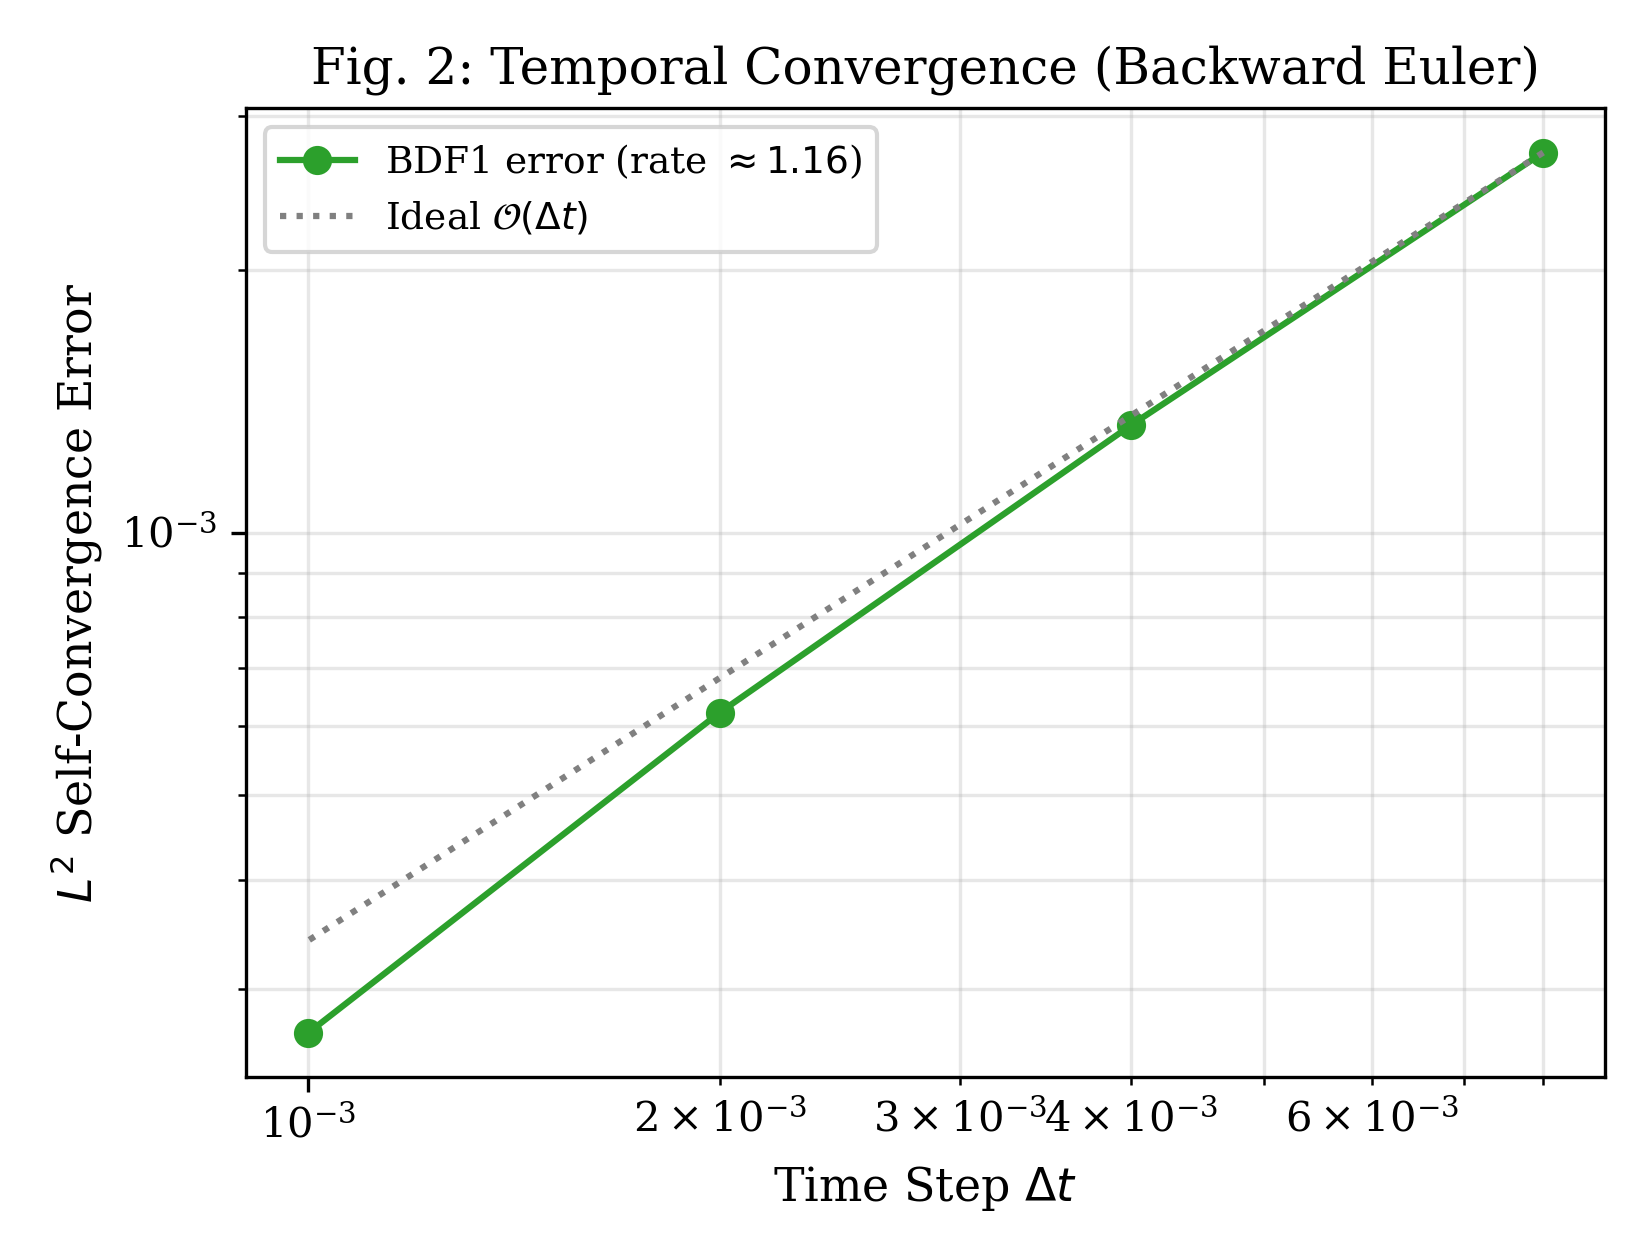
\includegraphics[width=0.90\linewidth]
    {images/stage_b/fig2_temporal_convergence.png}
    \caption{Convergenza temporale del solutore Backward Euler nello Stage B.}
    \label{fig:stage_b_temporal}
\end{figure}

\subsubsection{Diagnostica dell'accoppiamento GNN--PDE e dell'impatto del trasferimento di stato}

Dopo aver isolato il comportamento degli operatori su singoli eventi di trasferimento, viene valutato l'impatto dell'accumulo dell'errore durante l'evoluzione transiente della PDE descritta nella Sezione~\ref{subsec:pde_governing}. Questa campagna diagnostica non costituisce il benchmark comparativo finale dell'intero framework, ma mira a rispondere a una domanda metodologica specifica: l'errore aggiuntivo osservato con mesh mobile è associato principalmente alla configurazione geometrica prodotta dalla GNN oppure al meccanismo di trasferimento dello stato?

A tale scopo vengono confrontate la discretizzazione su mesh fissa e tre configurazioni dinamiche con intervallo di adattamento $N_a=10$ passi temporali, caratterizzate da differenti meccanismi di trasferimento.

\begin{table}[htbp]
\centering
\small
\setlength{\tabcolsep}{6pt}
\caption{Diagnostica dello Stage B: confronto dell'accuratezza PDE al tempo finale $T=0.5$ e dell'errore integrato nel tempo.}
\label{tab:stage_b_main}
\begin{tabular*}{\linewidth}{@{\extracolsep{\fill}}lcc@{}}
\toprule
Configurazione di verifica & $E_{L^2}(T)$ & $\overline{E}_{L^2}$ (time-integrated) \\
\midrule
Mesh fissa (riferimento Euleriano)  & $9.03\%$ & $7.96\%$ \\
GNN + remapping pointwise $P_1$    & $12.72\%$ & $10.32\%$ \\
GNN + proiezione $L^2$              & $8.99\%$ & $7.89\%$ \\
Oracle istantaneo + proiezione $L^2$ & $9.57\%$ & $8.35\%$ \\
\bottomrule
\end{tabular*}
\end{table}

La configurazione GNN + $P_1$ mostra un errore finale maggiore della mesh fissa, coerentemente con i risultati della diagnostica del trasferimento. Sostituendo il remapping pointwise con la proiezione $L^2$, l'errore finale scende a $8.99\%$, mentre l'errore integrato nel tempo risulta pari a $7.89\%$.

Nel benchmark considerato, lo scostamento rispetto alla mesh fissa rimane quindi contenuto. Il risultato più rilevante dello Stage B è la forte riduzione dell'errore aggiuntivo associato al trasferimento pointwise quando questo viene sostituito dalla proiezione $L^2$, a fronte del corrispondente incremento di costo computazionale.

Anche l'oracolo, quando accoppiato alla stessa proiezione $L^2$, restituisce un errore finale del $9.57\%$. Questo risultato conferma che l'oracolo introdotto nello Stage A deve essere interpretato come riferimento per la qualità geometrica istantanea e non come soluzione ottima del problema PDE transiente.

\paragraph{Gradiente FEM rispetto al gradiente analitico.}

Per verificare se la qualità dell'informazione fornita alla GNN dipenda in modo significativo dalla disponibilità della soluzione analitica, viene confrontato l'utilizzo del gradiente calcolato dal solutore FEM con quello analitico esatto.

La configurazione con gradiente FEM produce

\[
8.989\%
\]

di errore finale e

\[
7.890\%
\]

di errore integrato nel tempo, mentre il gradiente analitico produce rispettivamente

\[
8.979\%
\]

e

\[
7.889\%.
\]

La differenza è quindi molto ridotta nel benchmark considerato. Il risultato supporta l'impiego del gradiente FEM disponibile durante la simulazione come feature operativa della GNN, senza richiedere l'accesso alla soluzione analitica nella pipeline dinamica.

\paragraph{Sensibilità alla frequenza di adattamento.}

La frequenza di aggiornamento della mesh determina un compromesso tra accuratezza e costo computazionale. Considerando intervalli di adattamento pari a $5$, $10$, $20$ e $50$ passi temporali, si ottengono i risultati riportati in Tabella~\ref{tab:stage_b_frequency}.

\begin{table}[htbp]
\centering
\footnotesize
\setlength{\tabcolsep}{3pt}
\caption{Sensibilità dello Stage B alla frequenza di adattamento.}
\label{tab:stage_b_frequency}
\begin{tabular*}{\linewidth}{@{\extracolsep{\fill}}ccccc@{}}
\toprule
\begin{tabular}[c]{@{}c@{}}Intervallo\\ $N_a$\end{tabular} &
\begin{tabular}[c]{@{}c@{}}Adatt.\\ totali\end{tabular} &
\begin{tabular}[c]{@{}c@{}}Errore\\ $L^2(T)$\end{tabular} &
\begin{tabular}[c]{@{}c@{}}Errore\\ integrato\end{tabular} &
\begin{tabular}[c]{@{}c@{}}Tempo\\ tot. [s]\end{tabular} \\
\midrule
$5$  & $20$ & $8.984\%$ & $7.819\%$ & $9.50$ \\
$10$ & $10$ & $8.989\%$ & $7.890\%$ & $5.25$ \\
$20$ & $5$  & $9.001\%$ & $7.932\%$ & $3.11$ \\
$50$ & $2$  & $9.039\%$ & $7.957\%$ & $1.82$ \\
\bottomrule
\end{tabular*}
\end{table}

La riduzione della frequenza di adattamento diminuisce progressivamente il costo della simulazione, mentre l'errore varia solo moderatamente nel range considerato. Nel benchmark esaminato, l'aggiornamento della mesh a ogni passo temporale non risulta quindi necessario per mantenere un livello di accuratezza comparabile, introducendo un ulteriore parametro di controllo del costo della strategia adattiva.

\begin{figure}[H]
    \centering
    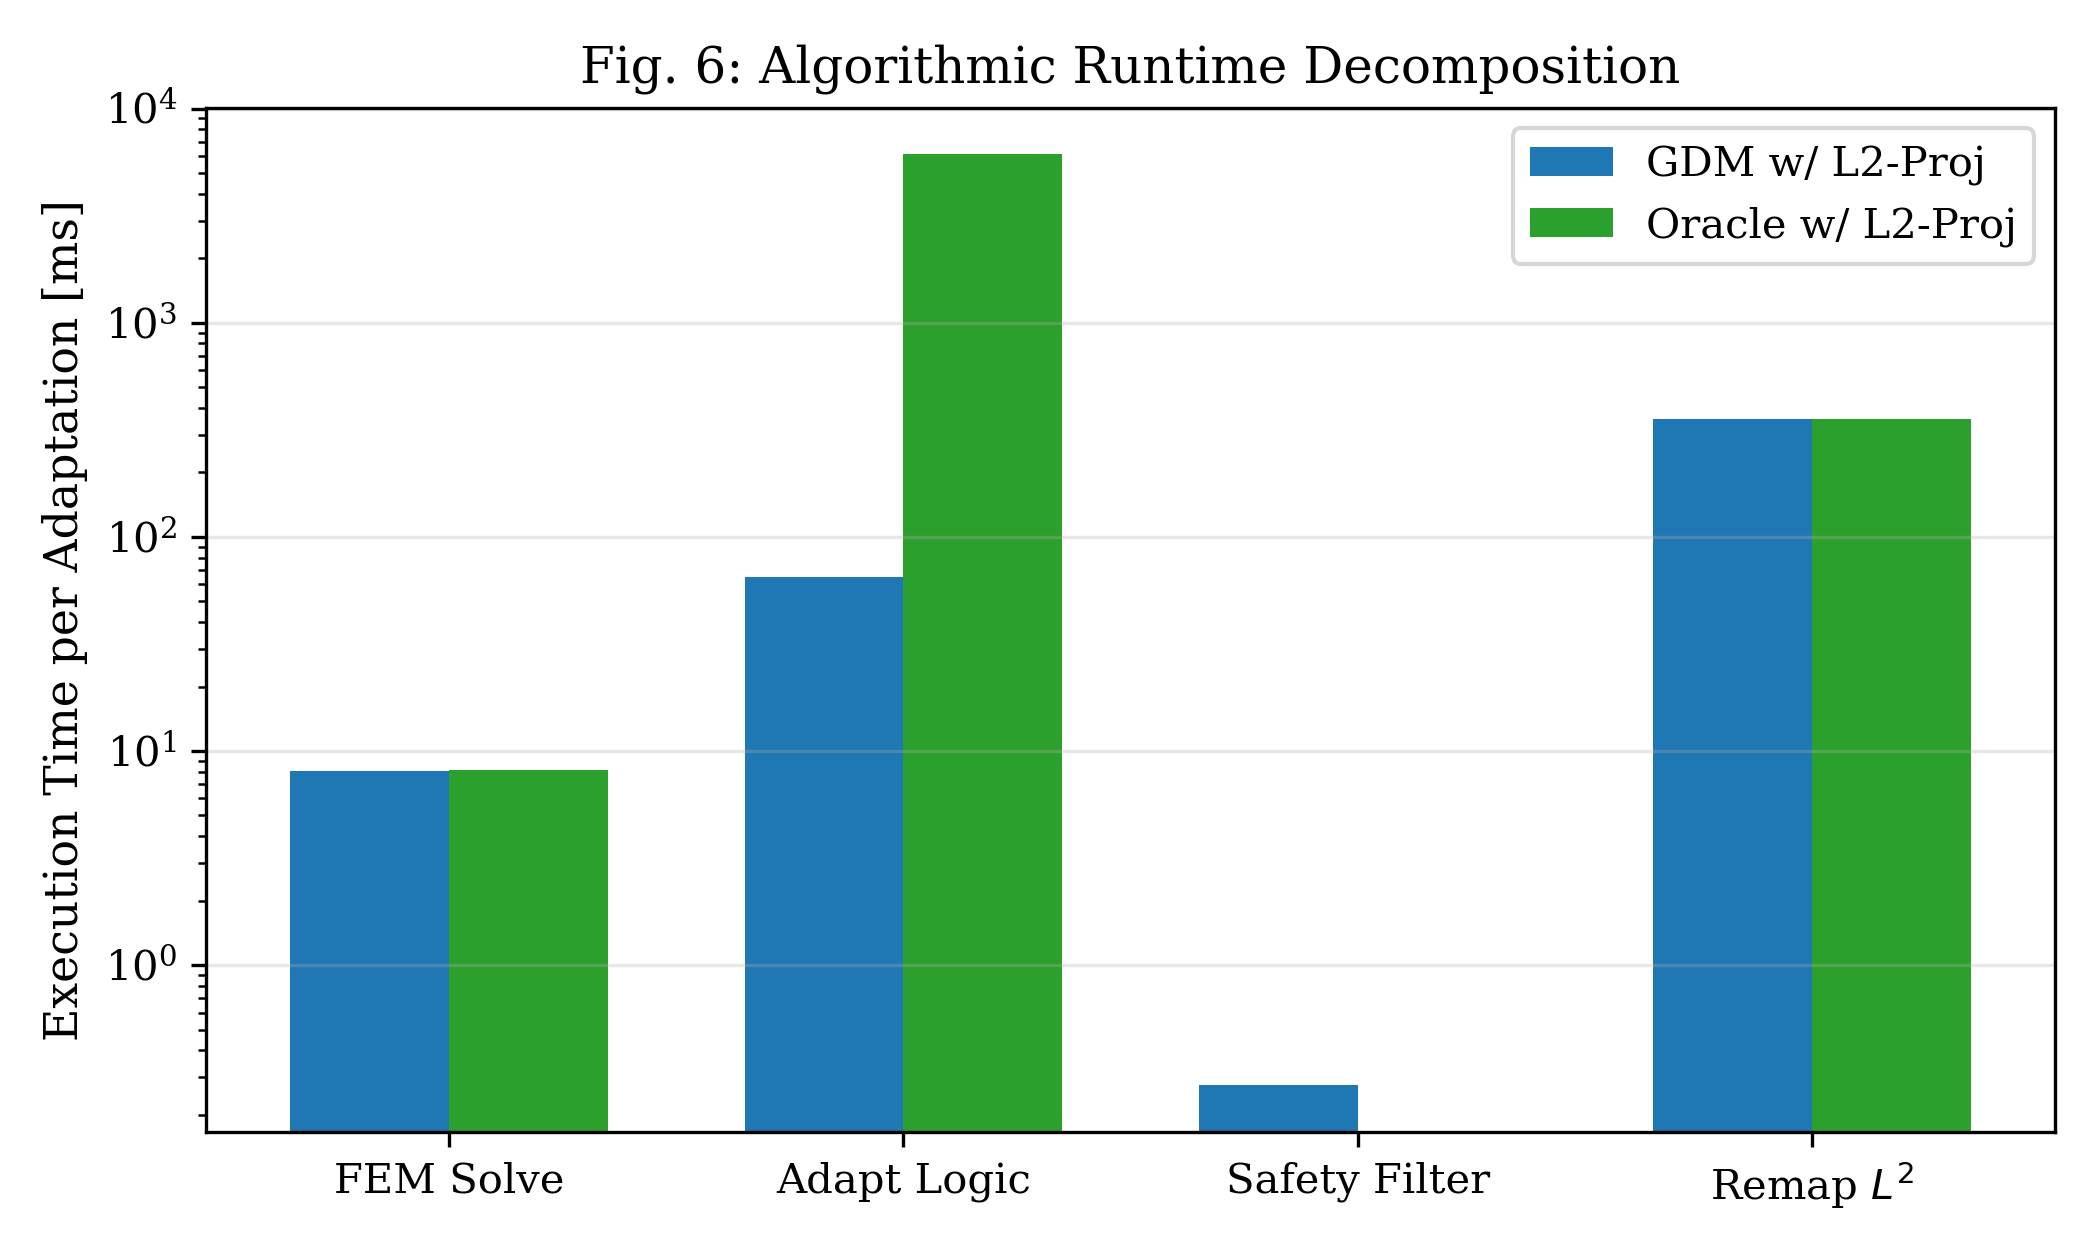
\includegraphics[width=0.95\linewidth]
    {images/stage_b/fig6_runtime_decomposition.png}
    \caption{Scomposizione del costo computazionale della simulazione dinamica nello Stage B.}
    \label{fig:stage_b_runtime}
\end{figure}

\begin{figure}[H]
    \centering
    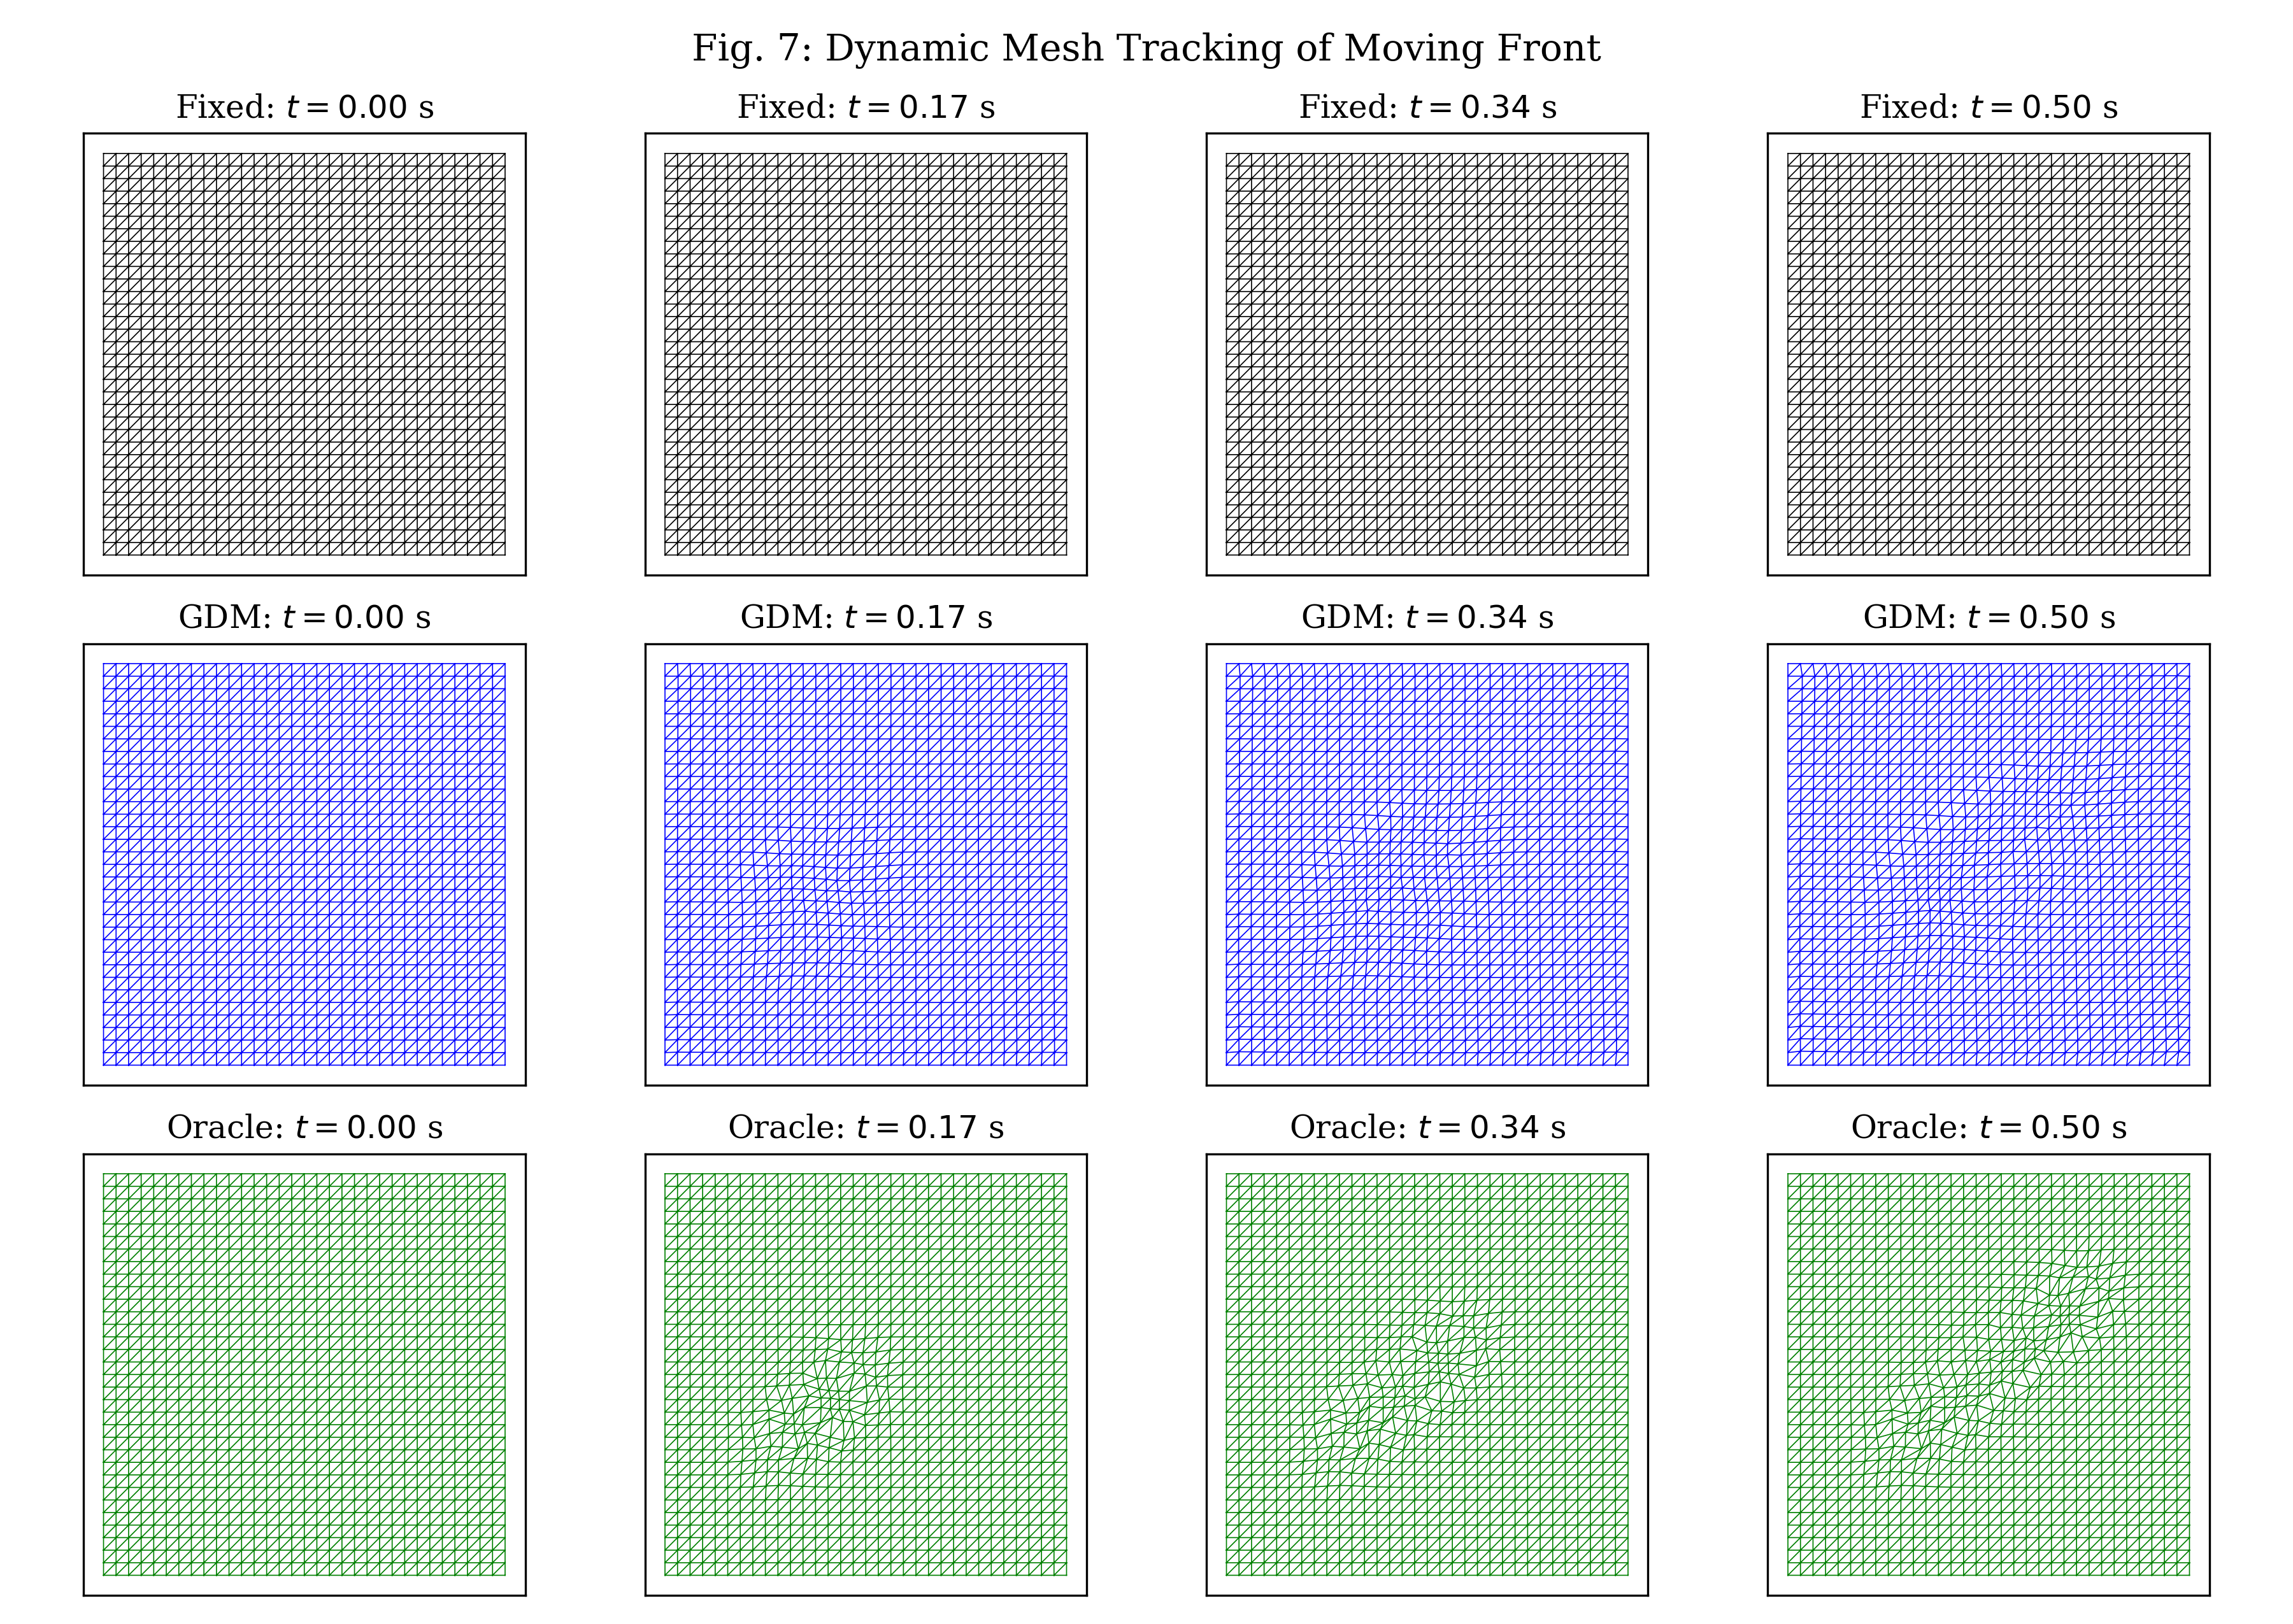
\includegraphics[width=0.95\linewidth]
    {images/stage_b/fig7_qualitative_dynamic_mesh.png}
    \caption{Evoluzione qualitativa della mesh adattata durante la simulazione transiente.}
    \label{fig:stage_b_mesh}
\end{figure}

\begin{figure}[H]
    \centering
    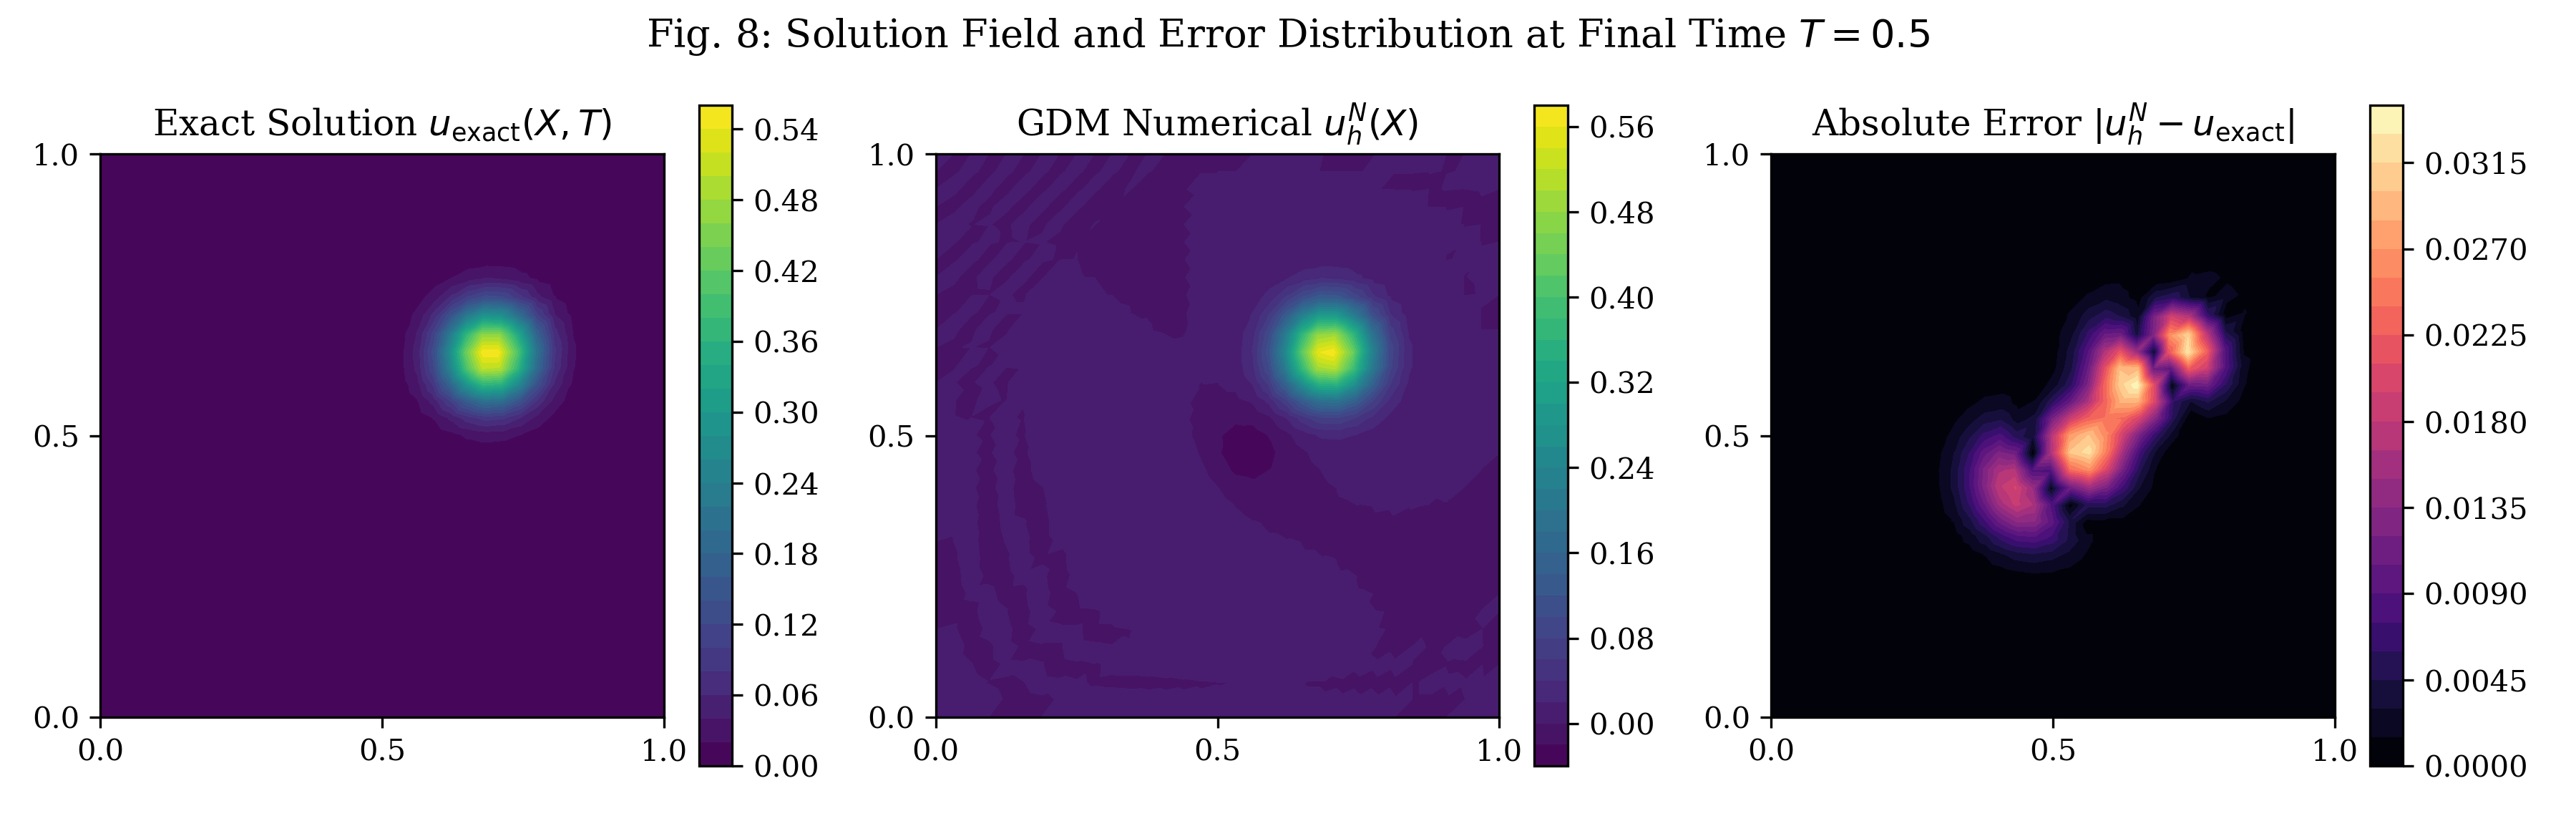
\includegraphics[width=0.90\linewidth]
    {images/stage_b/fig8_pde_error_field.png}
    \caption{Distribuzione spaziale dell'errore PDE nello Stage B.}
    \label{fig:stage_b_error_field}
\end{figure}

\paragraph{Conclusioni dello Stage B.}

Lo Stage B mostra che l'accuratezza globale di una simulazione a mesh mobile non può essere attribuita esclusivamente alla qualità della configurazione geometrica. Il trasferimento dello stato costituisce una componente numerica indipendente e può diventare rilevante quando viene ripetuto durante l'evoluzione temporale.

La proiezione $L^2$ riduce in modo significativo l'errore associato al trasferimento rispetto al remapping pointwise nel benchmark considerato, ma introduce un costo computazionale sensibilmente maggiore. Questa evidenza motiva il passaggio a una formulazione nella quale il moto della mesh viene incorporato direttamente nell'equazione differenziale.

\subsection{Verifica ALE e D-GCL: Stage C}

\label{subsec:stage_c_verification}

Lo Stage C introduce la formulazione ALE descritta nella Sezione~\ref{subsec:ale_formulation}. A differenza dello Stage B, nel quale ogni aggiornamento discreto della mesh richiede un trasferimento esplicito dello stato, lo spostamento prodotto dalla GNN viene distribuito su una finestra temporale e trasformato in una velocità di mesh continua a tratti.

Prima di utilizzare la formulazione ALE nel benchmark dinamico finale, vengono eseguiti cinque test indipendenti, indicati come C1--C5. Tali test verificano separatamente la cinematica della mesh, la consistenza geometrica, l'effetto della deformazione sulla soluzione PDE e il mantenimento degli ordini di convergenza spaziale e temporale.

\subsubsection{Test C1: verifica cinematica della velocità di mesh}

\label{subsubsec:c1}

Il primo test verifica la corrispondenza tra lo spostamento nodale prescritto e la velocità discreta

\[
\mathbf{w}^{n+\frac12}
=
\frac{\mathbf{X}^{n+1}-\mathbf{X}^{n}}{\Delta t}.
\]

Nel test considerato, l'errore relativo $L^2$ sulla velocità di mesh è

\[
1.64\times10^{-4},
\]

mentre l'errore $L^\infty$ è

\[
3.97\times10^{-5}.
\]

Il risultato mostra che la discretizzazione cinematica utilizzata dal solutore ALE rappresenta con errore contenuto il movimento nodale imposto.

\subsubsection{Test C2: verifica della D-GCL e preservazione del free stream}

\label{subsubsec:c2}

La consistenza geometrica discreta dello schema ALE viene verificata mediante gli indicatori introdotti nella Sezione~\ref{subsec:dgcl} su una sequenza di $100$ passi temporali deformanti.

Il massimo residuo geometrico element-wise risulta

\[
\max_{n,e}R_e^{\mathrm{GCL}}
=
4.34\times10^{-17},
\]

mentre il residuo della relazione matriciale discreta risulta

\[
\max_n
R_{\mathrm{alg}}^{\mathrm{GCL}}
=
5.42\times10^{-17}.
\]

Entrambi i valori sono prossimi alla precisione di macchina e indicano una forte consistenza numerica tra la variazione geometrica degli elementi e la discretizzazione della velocità di mesh.

La verifica del free stream, ottenuta imponendo un campo costante $u_0\equiv1$, fornisce

\[
E_{\mathrm{FS}}
=
2.81\times10^{-14}.
\]

Il campo uniforme rimane quindi invariato entro un errore prossimo alla precisione numerica del calcolo.

Nel complesso, i tre indicatori forniscono una verifica indipendente e coerente della D-GCL per la discretizzazione considerata. Il risultato viene interpretato come soddisfacimento della consistenza geometrica entro la precisione numerica osservata; non viene invece utilizzato come prova di una proprietà generale di conservazione fisica della PDE.

\subsubsection{Test C3: consistenza a singolo passo mediante MMS}

\label{subsubsec:c3}

Il test C3 confronta la soluzione ottenuta mediante un singolo passo su mesh fissa con quella ottenuta sulla configurazione deformata mediante il solutore ALE.

L'errore relativo $L^2$ risulta pari a

\[
4.0011\%
\]

per il caso di riferimento e

\[
4.1505\%
\]

per la configurazione ALE deformata.

La differenza è quindi pari a circa

\[
0.149
\]

punti percentuali.

Nel singolo passo considerato, la deformazione della mesh introduce pertanto un incremento limitato dell'errore complessivo rispetto alla configurazione fissa.

\begin{figure}[H]
    \centering
    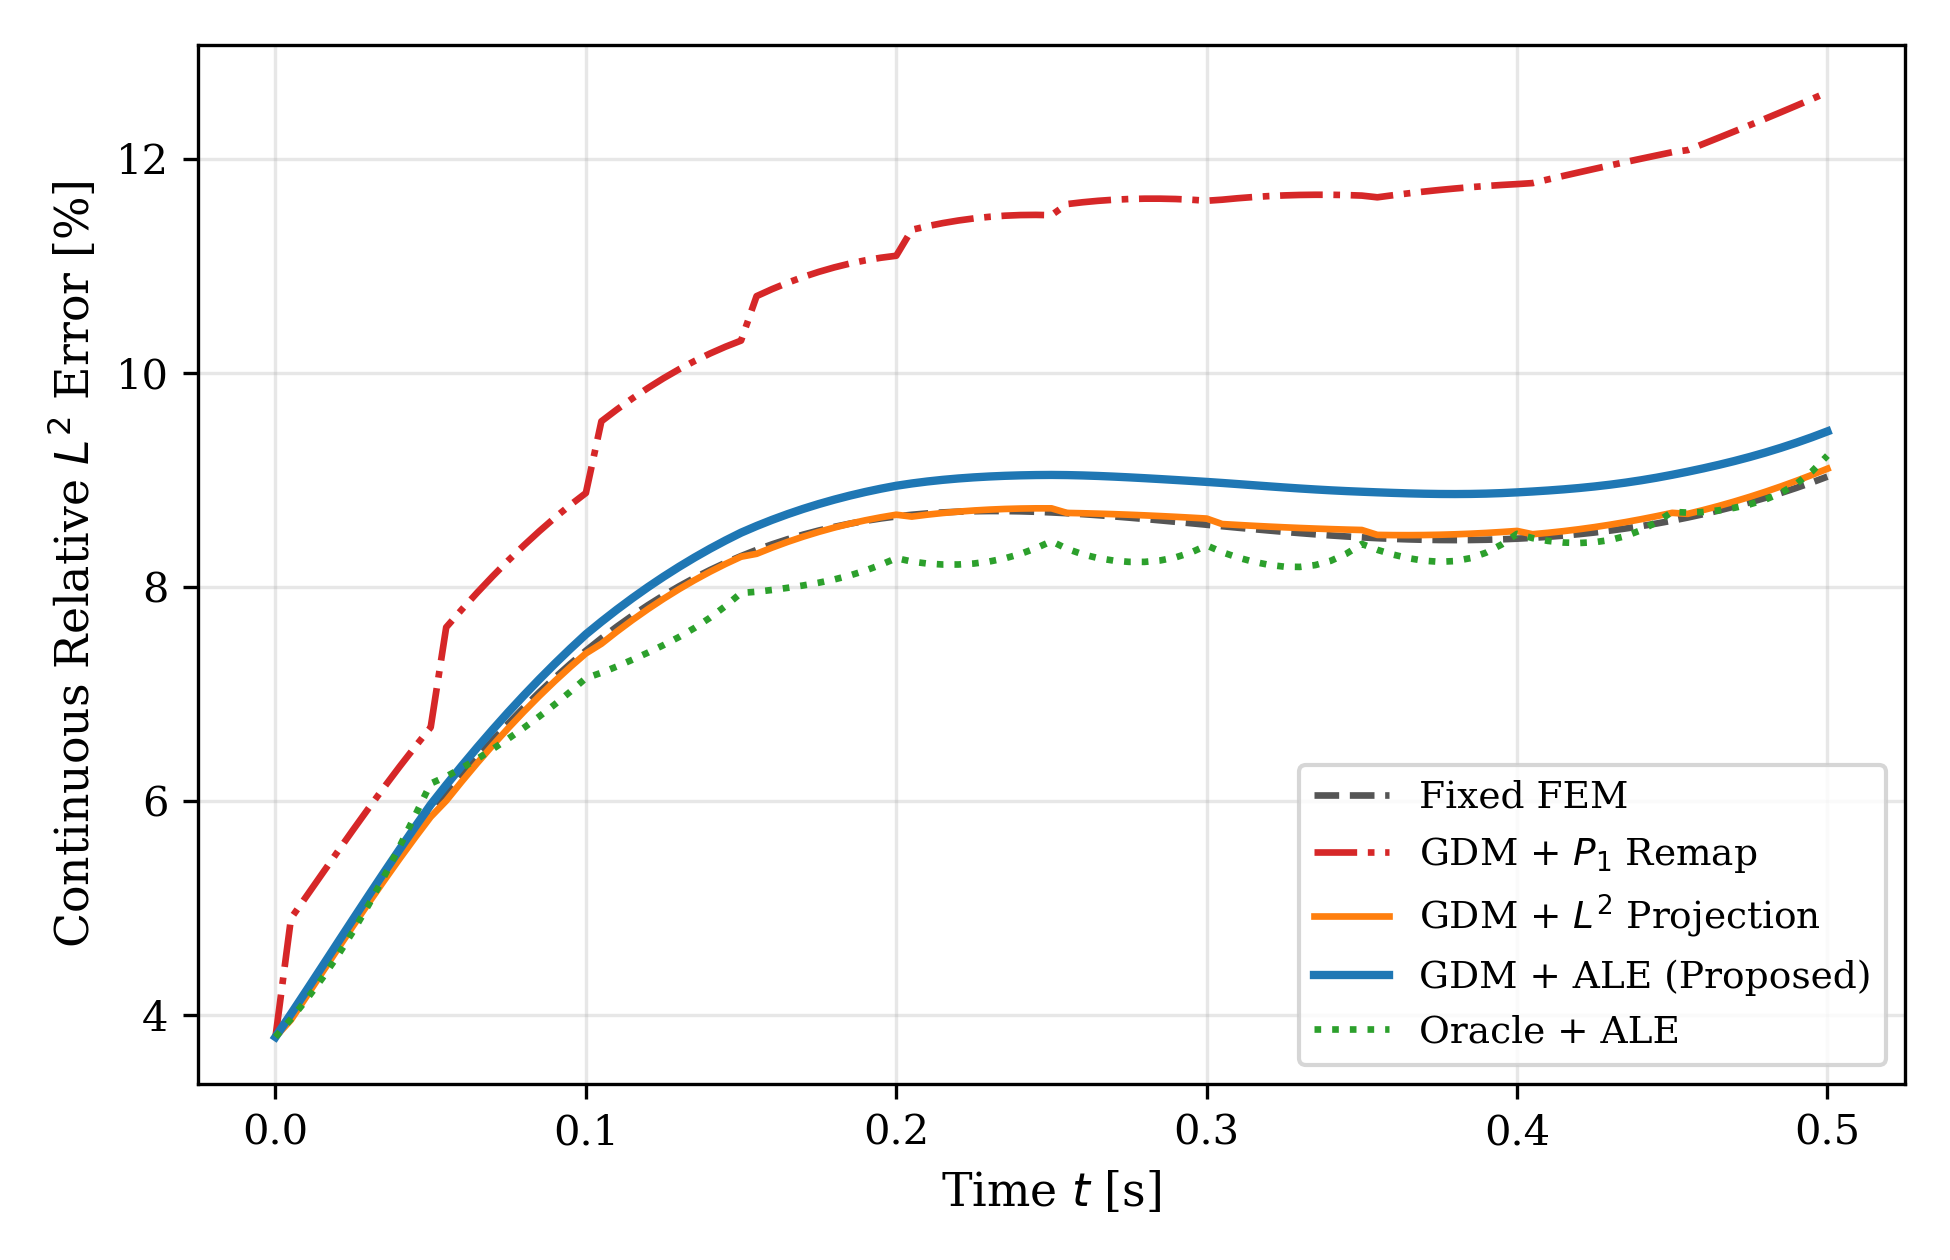
\includegraphics[width=0.90\linewidth]
    {images/stage_c/fig_c3_dynamic_error.png}
    \caption{Confronto dell'errore PDE nel test C3 tra configurazione fissa e configurazione ALE deformata.}
    \label{fig:stage_c_c3}
\end{figure}

\subsubsection{Test C4: convergenza spaziale su mesh deformate}

\label{subsubsec:c4}

Il test C4 verifica il comportamento della discretizzazione spaziale in presenza di mesh deformate, mantenendo la stessa topologia e aumentando progressivamente la risoluzione della griglia. L'errore viene misurato nelle norme $L^2$ e $H^1$ rispetto alla soluzione manufactured.

Per le risoluzioni considerate si ottengono i valori riportati in Tabella~\ref{tab:stage_c_spatial_convergence}.

\begin{table}[htbp]
\centering
\small
\setlength{\tabcolsep}{5pt}
\caption{Convergenza spaziale del solutore ALE su mesh deformate.}
\label{tab:stage_c_spatial_convergence}
\begin{tabular}{ccccc}
\toprule
Mesh & $E_{L^2}$ & Rate $L^2$ & $E_{H^1}$ & Rate $H^1$ \\
\midrule
$8\times8$   & $3.7062\times10^{-1}$ & --   & $7.1340\times10^{-1}$ & --   \\
$16\times16$ & $1.4345\times10^{-1}$ & $1.37$ & $4.5983\times10^{-1}$ & $0.63$ \\
$32\times32$ & $3.8812\times10^{-2}$ & $1.89$ & $2.4297\times10^{-1}$ & $0.92$ \\
$64\times64$ & $9.9228\times10^{-3}$ & $1.97$ & $1.2323\times10^{-1}$ & $0.98$ \\
\bottomrule
\end{tabular}
\end{table}

Gli ordini osservati tendono progressivamente ai valori attesi per elementi lineari $P_1$:

\[
\mathcal{O}(h^2)
\qquad\text{in }L^2,
\]

e

\[
\mathcal{O}(h)
\qquad\text{in }H^1.
\]

In particolare, sulle due ultime finestre di raffinamento vengono osservati ordini pari a $1.89$ e $1.97$ in norma $L^2$, e $0.92$ e $0.98$ in norma $H^1$. Il comportamento indica che la deformazione della mesh non impedisce il recupero del regime asintotico atteso nel range di risoluzioni considerato.

\subsubsection{Test C5: convergenza temporale per auto-convergenza}

\label{subsubsec:c5}

La convergenza temporale viene verificata mediante un test di auto-convergenza di tipo Cauchy utilizzando tre valori del passo temporale:

\[
\Delta t
=
0.01,\quad
0.005,\quad
0.0025.
\]

Le differenze tra soluzioni a passi successivi sono rispettivamente

\[
6.4654\times10^{-3},
\qquad
3.2591\times10^{-3},
\qquad
1.6482\times10^{-3},
\]

con ordini sperimentali pari a

\[
0.99
\qquad\text{e}\qquad
0.98.
\]

Il comportamento osservato è quindi compatibile con il primo ordine temporale atteso per Backward Euler,

\[
\mathcal{O}(\Delta t).
\]

\subsubsection{Sintesi della validazione Stage C}

Nel loro insieme, i test C1--C5 verificano separatamente le proprietà necessarie prima dell'introduzione della formulazione ALE nel benchmark dinamico finale:

\begin{itemize}
    \item C1 verifica la correttezza cinematica della velocità di mesh;
    \item C2 verifica la D-GCL elementare e algebrica e la preservazione del free stream;
    \item C3 quantifica l'effetto immediato della deformazione sulla soluzione PDE;
    \item C4 verifica il recupero degli ordini spaziali attesi della discretizzazione $P_1$ su mesh deformate;
    \item C5 verifica il primo ordine temporale della discretizzazione Backward Euler.
\end{itemize}

Nel complesso, i test mostrano che il solutore ALE conserva, nel regime esaminato, il comportamento di consistenza e convergenza della discretizzazione di riferimento anche in presenza di mesh deformate.

\paragraph{Sintesi complessiva della validazione.}

La sequenza Stage A--C permette di isolare progressivamente tre livelli del problema. Lo Stage A verifica che la GNN possa produrre deformazioni utili e che tali deformazioni possano essere sottoposte a un controllo geometrico deterministico. Lo Stage B mostra che, una volta inserito il movimento in una simulazione PDE transiente, il trasferimento dello stato costituisce una sorgente indipendente di errore e costo. Lo Stage C verifica quindi che il passaggio a una descrizione ALE continua sia compatibile con la discretizzazione FEM, con la D-GCL e con gli ordini di convergenza osservati.

Il significato dei tre stadi è quindi distinto: lo Stage A valuta la capacità di adattamento geometrico, lo Stage B quantifica il compromesso tra accuratezza e costo dei differenti operatori di trasferimento, mentre lo Stage C verifica la consistenza della formulazione ALE prima del confronto end-to-end.

Il confronto finale tra la strategia basata sulla proiezione $L^2$ e quella basata sulla formulazione ALE viene pertanto demandato al benchmark dinamico del capitolo successivo, dove le diverse pipeline vengono valutate con metriche comuni di accuratezza, costo computazionale e robustezza geometrica.
